\documentclass{article}
\DeclareMathAlphabet{\mathpzc}{OT1}{pzc}{m}{it}
\setlength{\parindent}{0pt}
\usepackage[table]{xcolor}
\usepackage{graphicx}
\usepackage{amssymb}
\usepackage{amsmath}
\usepackage{amsthm}
\usepackage{hyperref}
\usepackage{pgfplots}
\usepackage{pst-plot}
% \usepackage{fdsymbol}
\usepackage{empheq}
\usepackage{tikz}
\usepackage[most]{tcolorbox}
\usepackage{enumerate}
\usepackage{scalerel}
\usepackage{relsize}
\usepackage{mdframed}
\usepackage[utf8]{inputenc}

\usetikzlibrary{calc,patterns,angles,quotes}
\definecolor{myblue}{rgb}{2.55, 1.50, 0.20}
% \definecolor{myblue}{RGB}{227, 234, 253}
\newtcbtheorem[number within=subsection]{mytheo}{Sats}%
    {colback=myblue!15,colframe=black!30!black,
     enhanced,
     coltitle=black!75!black, boxrule=0.8pt,
     attach boxed title to top left=
       {xshift=2ex,yshift=-2mm,yshifttext=-1mm},
     boxed title style={colframe=black!30!black, boxrule=0.8pt,
       colback=myblue!60}}{th}

\newtcbtheorem[number within=subsection]{mydef}{Definition}%
    {colback=myblue!15,colframe=black!30!black,
     enhanced,
     coltitle=black!75!black, boxrule=0.8pt,
     attach boxed title to top left=
       {xshift=2ex,yshift=-2mm,yshifttext=-1mm},
     boxed title style={colframe=black!30!black, boxrule=0.8pt,
colback=myblue!60}}{th}

\newtcbtheorem[number within=subsection]{mykol}{Korollarium}%
    {colback=myblue!15,colframe=black!30!black,
     enhanced,
     coltitle=black!75!black, boxrule=0.8pt,
     attach boxed title to top left=
       {xshift=2ex,yshift=-2mm,yshifttext=-1mm},
     boxed title style={colframe=black!30!black, boxrule=0.8pt,
colback=myblue!60}}{th}

\newtcbtheorem[number within=subsection]{mylemma}{Lemma}%
    {colback=myblue!15,colframe=black!30!black,
     enhanced,
     coltitle=black!75!black, boxrule=0.8pt,
     attach boxed title to top left=
       {xshift=2ex,yshift=-2mm,yshifttext=-1mm},
     boxed title style={colframe=black!30!black, boxrule=0.8pt,
colback=myblue!60}}{th}

% ---------------------------------------------
% ---------------RE-NEW COMMAND----------------
% ---------------------------------------------
\newcommand\mul[1]{\multicolumn{1}{c}{#1}}
\setlength{\parskip}{1em}
\renewcommand{\baselinestretch}{1.2}
\renewcommand*{\proofname}{Bevis}
\newcommand{\ovning}[1]{\noindent {\bf Övning #1.}}
\renewcommand{\contentsname}{Innehåll}
\newcommand{\orbit}[0]{\mathlarger{\mathlarger{\mathcal{O}}}}
\newtheorem{definition}{Definition}[section]
\pgfplotsset{compat=1.8}

\theoremstyle{definition}
\newtheorem{thm}{Theorem}[section]
\newtheorem{exmp}[thm]{Exempel}
\begin{document}
% \pagecolor[HTML]{fefcf5}
% \pagecolor[HTML]{fffae6}
% ---------------------------------------------
% ---------------FÖRSTA SIDAN------------------
% ---------------------------------------------
\title{\LARGE{\textbf{Banach-Tarski paradoxen}}}
\author{Gabriel Rajkowski}
\date{\today}

\maketitle

\thispagestyle{empty}

\clearpage
\tableofcontents
\section{Inledning}
Syfte: Ta upp grunderna inom mängdlära, linjär algebra och gruppteori (med hubudfokus på gruppteori) 
så att läsaren ska känna sig tillräckligt matematisk mogen för att läsa vidare om mer avancerade grejer inom abstrakt algebra.
Syftet är även att bevisa Banach-Tarski paradoxen och ta upp detaljerna som andra källor, wikipedia, inte tar upp.

Frågeställningar: Går det att duplicera en cirkel istället för en sfär (ganska trivial)?
Går det att göra om en 2-sfär (2D-sphere, "3D sfär") till en 3-sfär ("4D sfär")
(ganska trivial)? Fungerar Banach-Tarski paradoxen i högre dimensioner (ganska trivial)?
Denna ovannämnda Frågeställningar skulle jag kunna besvara på direkt i sektionen
om Banach-Tarski paradoxen direkt efter beviset. En annan lämplig frågeställning skulle 
kunna vara "Går det att förstå paradoxen utan att använda matematik?". Här 
skulle jag kunna visa ett oformellt, men intuitivt, bevis av paradoxen utan att 
använda matematik överhuvudtaget. 

\section{Historia}
Här ska jag berätta mer om Stefan Banach och Alfred Tarski.
\section{Mängdlära}
Mängdläran studerar mängder och är en av matematikens grundstenar. 
\linebreak
Mängläraren är egentligen inte en del av
matematiken utan snarare en förutsättning för matematiken, vilket gör den intressant att studera.

En \textit{mängd} (eng. \textit{set}) är helt enkelt en samling av objekt eller \textit{element} där repetiition 
inte förekommer och ordningen inte har någon betydelse.
Dessa element kan vara vad som helst, vänner, bilar, nummer eller så kan dem själva vara mängder. 
Ett exempel på en mängd är 
\[S = \{\clubsuit, \diamondsuit, \spadesuit, \heartsuit\},\]
och vi skriver
\[\clubsuit, \diamondsuit, \spadesuit, \heartsuit \in S\]
för att indikera att $\clubsuit, \diamondsuit, \spadesuit, \heartsuit$ tillhör $S$.
Ibland kan mängder också vara tomma, det vill säga $\{ \}$. En sådan mängd kallas för en \textit{tom mängd} och 
betecknas med $\emptyset$. \textit{Kardinaliteten} av en mängd är storleken, det vill säga 
hur många element som finns i den, och betecknas med absolutbelopp. 
Kardinaliteten av exempelvis $S$ ges av
$|S| = 4$ och kardinaliteten av den tomma mängden är självklart noll. 

Mängder behöver dock inte alltid vara ändliga. 
Nedanför följer exempel på oändliga och vanliga mängder som majoriteten redan har 
stött på.
\begin{align*}
    \mathbb{N} & = \{0, 1, -1, 2, -2, \ldots \}, \\
    \mathbb{Z^+} & = \{1, -1, 2, -2, 3, -3, \ldots \}, \\
    \mathbb{Q} & = \{\frac{1}{2}, \ldots, -3, \ldots, 4, \ldots \}.
\end{align*}

Vi ser direkt att de rationella talen $\mathbb{Q}$ blir krångliga att skriva som en mängd. I 
dessa fall så kan man ta hjälp av \textit{mängdbyggare} för att beteckna en mängd. 
Ett bättre sätt 
att skriva de rationella talen med hjälp av mängdbyggare är på följande vis
\[ \mathbb{Q} = \biggl\{ \frac{m}{n} \; \biggl| \; m, n \in \mathbb{Z} \land n \neq 0 \biggl\}\]
som med ord blir \textit{mängden av de rationella talen innehåller $\frac{m}{n}$ så att $m, n$ är heltal och 
$n$ får inte vara noll.} Kort sagt så finner man
alltid elementen på vänstra sidan om $|$ och kriterierna som elementen måste uppfylla på högra sidan när man 
använder denna notation. Som exempel så kan man skriva mängden av alla jämna tal på följande vis
\[2 \mathbb{Z} = \{x \; | \; x = 2n, n \in \mathbb{Z}\} = \{0, 2, -2, 4, -4, \ldots\}.\]
Alla saker på mitt skrivbord kan också beskrivas som en mängd. Denna mängd kan skrivas som
\[ \textnormal{alla saker på mitt skrivbord} = \{x \; | \; x \in \textnormal{ mitt skrivbord}\}. \]
Vi definerar nu vad en delmängd är.

\begin{mydef}{}{}
  Mängden $A$ är en \textit{delmängd} (eng. \textit{subset}) av mängden $B$ om alla element i $A$ ingår även i $B$. Detta skrivs 
  $A \subseteq B$. Om $A \subseteq B$ och $A \neq B$ så är $A$ en \textit{äkta delmängd} (eng. \textit{proper subset}) av $B$ och skrivs
  $A \subset B$.
\end{mydef}
Vi ser direkt att $\emptyset \subseteq A$ för varje mängd $A$ och att varje mängd är en delmängd av 
sig själv. Definitionen medför även att om 
$A \subseteq B$ och $B \subseteq A$ så måste $A = B$, vilket vi kommer att avnända vid sxenare tillifällen för bevisföring. 

\begin{exmp}
Mängden $A = \{1, 2\}$ en 
äkta delmängd av $B = \{1, 2, 3, 4\}$ eftersom alla element som finns i $A$ finns även i $B$ och 
$A \neq B$. Därimot så
är $B$ inte en delmängd av $A$ eftersom $B$ innehåller element som inte finns i $A$.
\end{exmp}
 
Det går 
även att skriva dessa delmängder i "kedjor", till exempel 
$\mathbb{N} \subset \mathbb{Z} \subset \mathbb{Q} \subset \mathbb{R} \subset \mathbb{C}$, som
bilden på nästa sida försöker illustrera. 


%ta upp disktjunkta mängder

\begin{center}
  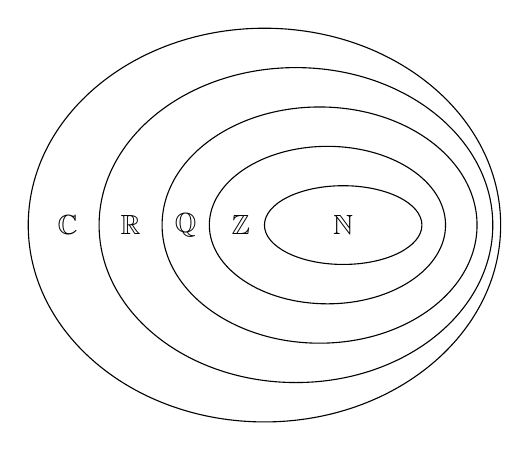
\begin{tikzpicture}
    \draw (0,0) ellipse (3cm and 2.5cm);
    \draw (0.4,0) ellipse (2.5cm and 2cm);
    \draw (0.7,0) ellipse (2cm and 1.5cm);
    \draw (0.8,0) ellipse (1.5cm and 1cm);
    \draw (1,0) ellipse (1cm and 0.5cm);
    \node[] at (-2.5,0) {$\mathbb{C}$};
    \node[] at (-1.7,0) {$\mathbb{R}$};
    \node[] at (-1,0) {$\mathbb{Q}$};
    \node[] at (-0.3,0) {$\mathbb{Z}$};
    \node[] at (1,0) {$\mathbb{N}$};
  \end{tikzpicture}
\end{center}

\subsection{Mängdoperationer}
Vi definerar nu några vanliga mängdoperationer som kommer att användas genom hela texten. 

\begin{mydef}{}{}
  \textit{Unionen} (eng. \textit{union}) av två mängder $A$ och $B$ är mängden av element som finns i 
  $A$ \textbf{eller} $B$ och betecknas med $\cup$. Med symboler blir definitionen
  \[A \cup B \equiv \{x \; | \; x \in A \; \lor \; x \in B  \}.\]
  Om $\mathpzc{A}$ är en mängd vars element är mängder så är $\bigcup \mathpzc{A}$ unionen
  av alla element i $\mathpzc{A}$. 
\end{mydef}

\begin{center}
  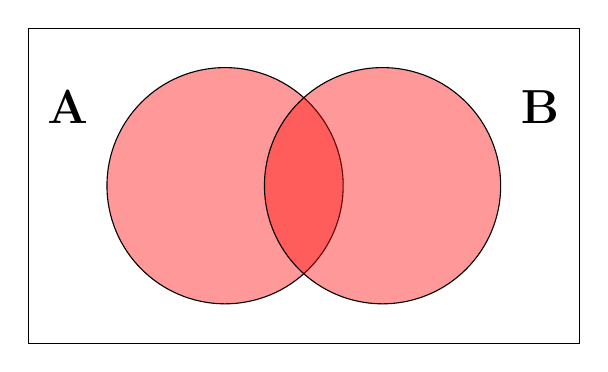
\begin{tikzpicture}
    \begin{scope} [fill opacity = .4]
      \draw[fill=red, draw = black] (-1,0) circle (1.5);
      \draw[fill=red, draw = black] (1,0) circle (1.5);
    \end{scope}
    
    \draw (-3.5,2) rectangle (3.5,-2);
    \node at (-3,1) {\LARGE\textbf{A}};
    \node at (3,1) {\LARGE\textbf{B}};
    % \node at (0,0) {\LARGE\textbf{O}};

      % \draw[help lines](-5,5) grid (5,-6);  
  \end{tikzpicture}
\end{center}
Det hela röda området i venn diagramet visar $A \cup B$. Man kan alltså tänka att unionen
av två mängder sammansätter de två mängderna.
\begin{exmp}
  Låt $A = \{1, 2, 3\}$ och $B = \{3, 4, 5\}$. Då är $A \cup B = \{1, 2, 3, 4, 5\}$ 
  eftersom repetition inte förekommer i mängder.   
\end{exmp}
För en union av flera mängder $A_1, A_2, \ldots, A_n$
kan det ibland bli jobbigt att skriva $A_1 \cup A_2 \cup \ldots \cup A_n$. Därför har man infört 
en ny beteckning för detta, nämligen $\bigcup\limits_{i=1}^{n} A_i$. 
% Om 
% $\mathpzc{A}$ istället är en mängd där elementen är mängder 
% (en sådan mängd brukar betecknas med en "fin" bokstav) så är $\bigcup 
% \mathpzc{A}$ unionen av alla element i $\mathpzc{A}$. 

\begin{mydef}{}{}
  \textit{Snittet} (eng. \textit{intersection}) av två mängder $A$ och $B$ är mängden av element som finns i $A$ \textbf{och} $B$ och
  betecknas med $\cap$. Med symboler blir definitionen
  \[A \cap B \equiv \{x \; | \; x \in A \; \land \; x \in B  \}.\]
  Om $\mathpzc{A}$ är en mängd vars element är mängder så är $\bigcap \mathpzc{A}$ 
  snittet av alla element i  $\mathpzc{A}$.
\end{mydef}

\begin{center}
  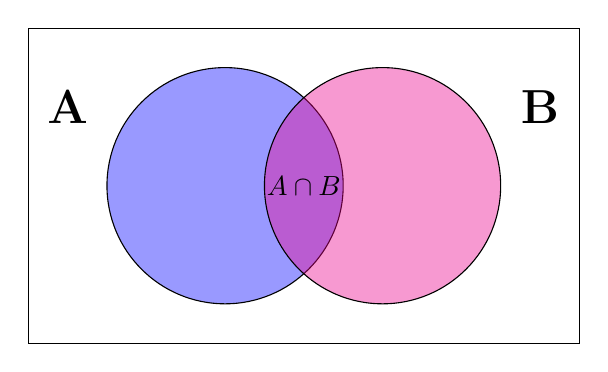
\begin{tikzpicture}
    \begin{scope} [fill opacity = .4]
      \draw[fill=blue, draw = black] (-1,0) circle (1.5);
      \draw[fill=magenta, draw = black] (1,0) circle (1.5);
    \end{scope}
    
    \draw (-3.5,2) rectangle (3.5,-2);
    \node at (-3,1) {\LARGE\textbf{A}};
    \node at (3,1) {\LARGE\textbf{B}};
    \node at (0,0) {\textbf{$A \cap B$}};

      % \draw[help lines](-5,5) grid (5,-6);  
  \end{tikzpicture}
\end{center}
Det lila området där cirklarna överlappar i venn diagramet visar $A \cap B$. Snittet 
av två mängder är alltså mängden av alla gemensamma element. 
\begin{exmp}
  Låt $A$ och $B$ vara mängder som förekom i förra exemplet, då är $A \cap B = \{3\}$.
\end{exmp}
Även här har man infört en ny beteckning för att slippa skriva mycket. Istället 
för att skriva $A_1 \cap A_2 \cap \ldots \cap A_n$ så kan man skriva $\bigcap\limits_{i = 1}^n A_n$.
% Om $\mathpzc{A}$ istället är en mängd vars element är mängder så är $\bigcap \mathpzc{A}$ snittet 
% av alla element i  $\mathpzc{A}$.

\begin{mydef}{}{}
  \textit{Differensen} (eng. \textit{relative complement}) av två mängder $A$ och $B$ är mängden av element som finns i $A$ 
  men som inte finns i $B$. Detta
  betecknas med $\setminus$ och utläses "$A$ utom $B$". Med symboler blir definitionen 
  \[A \setminus B \equiv \{x \; | \; x \in A, \; x \notin B  \}\]
\end{mydef}

\begin{center}
  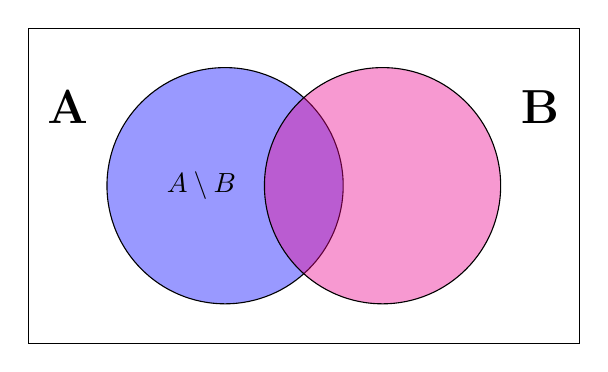
\begin{tikzpicture}
    \begin{scope} [fill opacity = .4]
      \draw[fill=blue, draw = black] (-1,0) circle (1.5);
      \draw[fill=magenta, draw = black] (1,0) circle (1.5);
    \end{scope}
    
    \draw (-3.5,2) rectangle (3.5,-2);
    \node at (-3,1) {\LARGE\textbf{A}};
    \node at (3,1) {\LARGE\textbf{B}};
    \node at (-1.3,0) {\textbf{$A \setminus B$}};

      % \draw[help lines](-5,5) grid (5,-6);  
  \end{tikzpicture}
\end{center}
Endast det blåa området (och inte det lila området där cirklarna överlappar) i venn diagramet
visar $A \setminus B$. Differensen mellan två mängder $A$ och $B$ är alltså mängden av element
som är unika i $A$. 

Notera att differensen mellan två mängder inte är kommutativ, det vill säga 
$A \setminus B \neq B \setminus A$.
\begin{exmp}
  Låt $A$ och $B$ vara mängder som förekom i förra exemplet, då är $A \setminus B
  = \{1, 2\}$.  
\end{exmp}
Det finns såklart fler operationer som kan utföras på mängder men 
\linebreak
dessa utelämnas i denna 
text. 
Operationerna som har tagits upp är de vanligaste och endast dessa kommer 
att användas framöver. Två saker till bör dock defineras innan detta del avsnitt avslutas. 

\begin{mydef}{}{}
  Två mängder $A$ och $B$ är \textit{disjunkta} om $A \cap B = \emptyset$. Om $\mathpzc{A}$ är 
  en mängd vars element är mängder så är $\mathpzc{A}$ \textit{parvis disjunkt} om $\bigcap \mathpzc{A} = 
  \emptyset$.
\end{mydef}
I ett venn diagram så skulle alltså $A$ och $B$ inte överlappa varandra
om det var disjunkta. 
\begin{exmp}
  Mängderna $A = \{1, 2, 3\}$ och $B = \{4, 5\}$ 
  är disjunkta eftersom $A$ och $B$ inte har några gemensamma element. 
  Om 
  \[\mathpzc{A} = \{\{1, 2, 3\}, \{4, 5, 6\}, \{7, 8, 9\}\ldots\}\] 
  så är $\mathpzc{A}$ parvis disjunkt eftersom alla element i mängden 
  inte har några gemensamma element. 
\end{exmp}

\begin{mydef}{}{}
  En \textit{partition} (eng. \textit{partition}) av en mängd $A$ är en mängd av icke-tomma delmängder av $A$ sådant att 
  varje element i $A$ endast förekommer en gång i dessa delmängder. 
  Partitionen av $A$ måste alltså vara parvis disjunkt.
\end{mydef}
%flytta alla exempel längdst ned??
\begin{exmp}
  Låt $A = \{1, 2, 3\}$. Denna mängd kan ha fem olika partitioner, nämligen
\begin{itemize}
  \item $\{\{1\}, \{2\}, \{3\}\}$,
  \item $\{ \{1, 2\}, \{3\} \}$,
  \item $\{ \{1, 3\}, \{2\} \}$,
  \item $\{ \{1\}, \{2, 3\} \}$.
  \item $\{ \{1, 2, 3\} \}$
\end{itemize}
Medan $ P = \{ \{\}, \{1, 2\}, \{4, 3, 2\} \}$ inte är en partition av $A$ på grund av några anledningar, $P$ innehåller en tom mängd, mängden $\{4, 3, 2\}$ är inte en delmängd till $A$
och $P$ är inte heller parvis disjunk, $\bigcup P = \{2\} \neq \emptyset$. Notera att det endast räcker med att nämna en av dessa anledningar för att visa att $P$ inte är en partition av $A$.
\end{exmp}

\subsection{Tuplar och ordnade par}
\begin{mydef}{Tuplar och ordnade par}{}
  En $n$\textit{-tupel} (eng. \textit{tuple}) är en sekvens innehållande $n$ styckna olika objekt, $(n_0, n_1, n_2, \ldots, n_n)$, där ordningen mellan dem spelar roll. Dessa objekt
  kallas för \textit{komponenter}. Ett \textit{ordnat par} (eng. \textit{ordered pair}) är ett annat namn för en 2-tupel.
\end{mydef}
Notera att en $n$-tupel skiljer sig från en mängd eftersom ordningen har betydelse.
\begin{exmp}
  (DAG, MÅNAD, ÅR) är en 3-tupel 
  eftersom den innehåller 
  en sekvens som består av tre styckna object där ordningen har betydelse. 
\end{exmp}

\begin{exmp}
  Punkter i ett kartesiskt eller polärt koordinatsystem är ordnade par
  eftersom för två olika $x$ och $y$ så är punkten $(x, y) \neq (y, x)$. 
\end{exmp}
% För bevisföring inom mängdläran 
% så kan man använda sig av Kuratowskis definition av ordande par som säger att 
% $(a, b) = \{ \{a\}, \{a, b\} \}$. 

\subsection{Kartesiska produkter}

\begin{mydef}{Kartesiska produkter}{}
  Den \textit{kartesiska produkten} av två mängder $A$ och $B$ är mängden av alla ordnade par $(a, b)$
  där $a \in A$ och $b \in B$. Kartesiska produkten tecknas med $A \times B$ och utläses "$A$ kryss $B$".
  Med symboler blir definitionen
  \[A \times B \equiv \{(a, b) \; | \; a \in A, \; b \in B\}.\]
\end{mydef}
%onödigt med detta. Ha kvar detta nedan om jag ska ha övningar i min text, eller ta bort 
%den så att läsaren får klura ut detta själv. 
Lägg märke till att $|A \times B|=|A| \cdot |B|$ eftersom varje elementen i $A$
måste accosieras med varje elementen i $B$.

\begin{exmp}
  Låt $A = \{13, 37, 0\}$ och $B = \{4, 2\}$. Då är
\[A \times B = \{ (13, 4), (13, 2), (37, 4), (37, 2), (0, 4), (0, 2) \},\]
medan 
\[B \times A = \{ (4, 13), (4, 37), (4, 0), (2, 13), (2, 37), (2, 0) \}.\]
Vi ser att $A \times B \neq B \times A$ eftersom ordningen
har betydelse i ordade par och därför är den kartesiska produkten inte kommutativ. 
\end{exmp}
För att konstruera en mängd med $3$-tuplar så kan följande göras.
\[A \times B \times C = \{ (a, b, c) \; | \; a \in A, \; b \in B, \; c \in C \},\]
där $A, B$ och $C$ är mängder. Detta konceptet kan generaliseras till $n$-tuplar. 
Den kartesiska produkten ger oss även ett sätt att "skapa" fler dimensioner.
%ett annat ord för skapa kanske?
$\mathbb{R} \times \mathbb{R}$ är alla möjliga ordnade par av de reella talen och skapar därför det 
tvådimensionella rummet $\mathbb{R}^2$. På samma sätt kan man skapa det tredimensionella rummet,
$\mathbb{R} \times \mathbb{R} \times \mathbb{R} = \mathbb{R}^3$, och konceptet kan generaliseras till 
$\mathbb{R}^n$. 
\[\mathbb{R}^n = \{(x_1, x_2, x_3, \ldots, x_n) \; | \; x_i \in \mathbb{R} \textnormal{ för } 1 
\leq i \leq n\; \} \].


% ta även upp att R X R är R^2 osv. här så att jag slipper göra det i linjär algebra delen.
\subsection{Axiomatiska system och Russells paradox}
Ibland kan det uppkomma olika paradoxer med mängder om man inte är försiktig. Det stora problemet 
ligger för det mesta att elementen i en mängd kan själva vara mängder. För att demonstrera en sådan 
paradox så kan vi ta Russells paradox som utvecklades under 1800-talet av den italienska logikern Burali-Forti
och senare av Bertrand Russell. 

Vi börjar med att definera en mängd $S$ som består av alla mängder $X$ sådana att $X$ inte innehåller 
$X$. Med symboler kan vi skriva denna mängd som
\[S = \{X \; | \; X \textnormal{ är en mängd och } X \notin X  \}. \]
För att åstadkomma paradoxen så ställer vi frågan om $S$ innehåller sig själv eller inte. 
Vi antar först att $S \in S$.
För att $S$ ska vara ett element av $S$ så 
måste $S$, per definition, vara en mängd och $S \notin S$.
Vi antog dock att $S \in S$, vilket betyder att $S \notin S$. Vi kontruerade dock $S$ på ett sådant sätt att om $S \notin S$ så betyder det samtidigt att $S \in S$ och vi hamnar i ett
cirkelresonemang på liknande vis som vid "påståendet" "detta påstående är falskt".

För att undvika dessa paradoxer så har tanken om mängdlära som ett axiomatiskt system växt fram. 
Idag finns det flera sådana system, till exempel Zermelo–Fraenkel systemet (ZF). Det vanligaste 
systemet är Zermelo–Fraenkel systemet kombinerat med Urvalsaxiomet (ZFC). Detta avnsitt har inte använts sig 
av ett sådant system eftersom det inte var nödvändigt. 
Urvalsaxiomet (eng. Axiom of Choice, AC) kommer dock att 
tas upp och diskuteras i detalj senare i texten.

\section{Funktioner}
För att förstå viktiga koncept inom gruppteori så måste vi definera en funktion mer formellt och ta upp detaljer som man vanligtvist soppar under mattan i en vanlig gymnasiekurs.

\begin{mydef}{Funktioner}{}
  En \textit{funktion} $f$ från den icke tomma mängden $X$, \textit{definitionsmängden}, till den icke tomma mängden $Y$, \textit{målmängden},är definerad 
  av en mängd $G$ av ordnade par $(x, y), x \in X, y \in Y$ så att $x$ är den första komponenten i \textbf{exakt ett} ordnat par i $G$ för att $x$. En funktion $f$ från mängden $X$
  till mängden $Y$ betecknas
  \[f: X \rightarrow Y.\]
  Om $(x, y) \in G$ så är $y$ värdet av $f$ av $x$ och skrivs $y=f(x)$. Mängden av alla möjliga utvärden av funktionen, det vill säga mängden av alla $f(x)$, är funktionens \textit{värdemängd}.
\end{mydef}

En funktion enligt denna definition är alltså en regel som till varje element i definitionsmängden kopplar alla element i värdemängden. Om definitionsmängden och värdemängden endast innehåller
tal så brukar man kunna beskriva denna regel med en matematisk formell, till exempel $f(x) = x^2$.

Intuitivt så är en funktion $f(x) = x^2$ en slags "maskin". Man stoppar in ett element från definitionsmängden i funktionen och på ett magiskt sätt så kommer det ut ett annat tal. Formellt så assocerar,
eller \textit{mappar}, en funktion ett element från definitionsmängden till ett korresponderande element från målmängden.


\begin{center}
  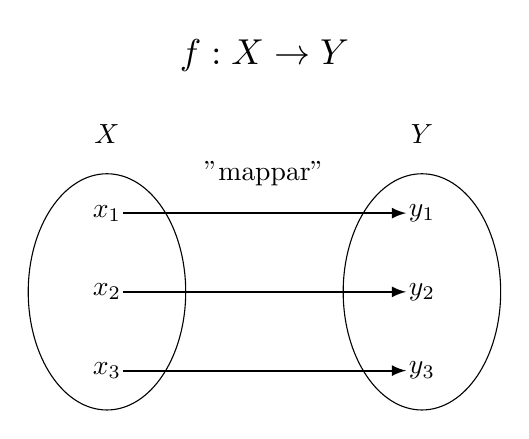
\begin{tikzpicture}
    \draw (0,0) ellipse (1cm and 1.5cm);
    \node at (0,1) {$x_1$};
    \node at (0,0) {$x_2$};
    \node at (0,-1) {$x_3$};
    \node at (0, 2) {$X$};

    \draw (4,0) ellipse (1cm and 1.5cm);
    \node at (4,1) {$y_1$};
    \node at (4,0) {$y_2$};
    \node at (4,-1) {$y_3$};
    \node at (4, 2) {$Y$};

    \draw [-latex, thick] (0.2, 1) -- (3.8, 1);
    \draw [-latex, thick] (0.2, 0) -- (3.8, 0);
    \draw [-latex, thick] (0.2, -1) -- (3.8, -1);

    \node at (2,1.5) {"mappar"};

    \node[scale=1.3] at (2, 3) {$f: X \rightarrow Y$};
  \end{tikzpicture}
\end{center}

De två cirklarna i figuren ovanför skall föreställa två mängder $X$ och $Y$. En funktion 
från $X$ till $Y$ mappar alltså ett element $x \in X$ med ett korresponderande element $y \in Y$
vilket skrivs $f: x \mapsto y$ och är ett annat sätt att definera denna funktion på istället för $f(x) = y$.
Funktionen defineras i detta fall av mängden $G = \{ (x_1, y_1), (x_2, y_2), (x_3, y_3) \}$ och dess 
definitionsmängd är $X = \{ x_1, x_2, x_3\}$ och målmängden är identisk med värdemängden, det vill säga $Y = \{ y_1, y_2, y_3\}.$ 

\begin{exmp}
  Betrakta funktionen $f(x) = x^2$ för $x \in \mathbb{R}$. Denna funktion mappar 
  ett reellt tal $x$ med $x^2$, vilket skrivs 
  $f: x \mapsto x^2$
  och är ett annat sätt att definera funktionen på.
  Eftersom funktionen mappar ett reellt tal med ett annat reellt tal så är definitionsmängden
  och målmängden $\mathbb{R}$, det vill säga 
  $f: \mathbb{R} \rightarrow \mathbb{R}.$
  Värdemängden är alla möjliga utvärden av funktionen och eftersom kvadraten av ett reellt tal alltid 
  är positivt så är värdemängden alla positiva reella tal. 
  Mängden som definerar $f(x) = x^2$ är
  $G = \{ (x, x^2) \; | \; x \in \mathbb{R}\}.$  
\end{exmp}

\begin{exmp}
  Vi avgör nu om $y^2 = x, \; x \in \mathbb{R}$ är en funktion eller inte. 
  Mängden 
  som definerar denna ekvation är $G = \{ (x^2, x) \; | \; x \in \mathbb{R} \}.$
  För att denna ekvation ska vara en funktion
  så måste $x^2, \; x \in \mathbb{R}$ vara den första komponanten i \textbf{exakt ett} ordnat par i $G$.
  Vi ser att $(1^2, 1) \in G$ och att $((-1)^2, -1) = (1^2, -1) \in G$. 
  $1^2$ förekommer i två ordnade par som den första komponenten och därför är 
  $y^2 = x$ inte en funktion.  
\end{exmp}

Notera att funktioner inte behöver gå från tal till tal. Definitionsmängden och målmängden är 
mängder och kan därför innehålla massor av olika saker. En funktion kan till exempel 
mappa en geometrisk figur med en färg, ett ansiktsuttryck med en känsla osv. 

\subsection{Bijektion, injektion och surjektion}
\begin{mydef}{}{}
  Låt oss definera funktionen
  \[f: X \rightarrow Y.\]
  \begin{itemize}
    \item $f$ är \textit{injektiv} om alla element i $Y$ är mappade med \textbf{högst}
    ett element från $X$, det vill säga det finns högts ett $x \in X$ så att $f(x) = y, \; y \in Y.$
    Med symboler och för bevisföring
    \[\forall x, x' \in X, f(x) = f(x') \implies x = x'.\]
    \item $f$ är \textit{surjektiv} om alla element från 
    $Y$ är mappade med \textbf{åtminstone} ett element från $X$, det 
    vill säga det finns åtminstone ett $x \in X$ så att $f(x) = y, \; y \in Y.$
    Med symboler och för bevisföring
    \[\forall y \in Y, \exists x \in X \; | \; y = f(x).\]
    \item $f$ är \textit{bijektiv} om alla element från värdemängden är mappade med \textbf{exakt} 
    ett element från definitionsmängden. Funktionen är alltså både injektiv och surjektiv.
    Med andra ord så existerar det endast ett $x \in X$ så att $f(x) = y, \; y \in Y.$
  \end{itemize}
\end{mydef}

\begin{exmp}
  Ellipserna i figuren nedan föreställer mängder.
\end{exmp}
\begin{center}
  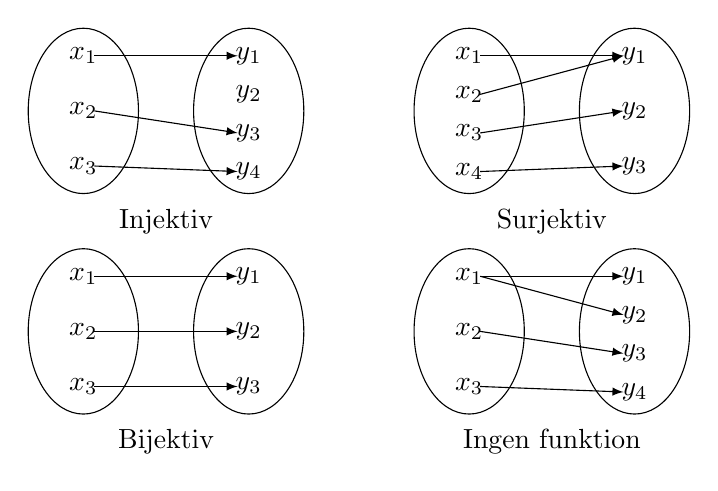
\begin{tikzpicture}[scale = 0.7]
    \draw (0,0) ellipse (1cm and 1.5cm);
    \node at (0, 1) {$x_1$};
    \node at (0, 0) {$x_2$};
    \node at (0, -1) {$x_3$};
    \draw (3,0) ellipse (1cm and 1.5cm);
    \node at (3, 1) {$y_1$};
    \node at (3, 0) {$y_2$};
    \node at (3, -1) {$y_3$};
    \draw [-latex] (0.2, 1) -- (2.8, 1);
    \draw [-latex] (0.2, 0) -- (2.8, 0);
    \draw [-latex] (0.2, -1) -- (2.8, -1);
    \node at (1.5, -2) {Bijektiv};

    \draw (7,0) ellipse (1cm and 1.5cm);
    \node at (7, 1) {$x_1$};
    \node at (7, 0) {$x_2$};
    \node at (7, -1) {$x_3$};
    \draw (10,0) ellipse (1cm and 1.5cm);
    \node at (10, 1) {$y_1$};
    \node at (10, 0.3) {$y_2$};
    \node at (10, -0.4) {$y_3$};
    \node at (10, -1.1) {$y_4$};
    \draw [-latex] (7.2, 1) -- (9.8, 1);
    \draw [-latex] (7.2, 1) -- (9.8, 0.3);
    \draw [-latex] (7.2, 0) -- (9.8, -0.4);
    \draw [-latex] (7.2, -1) -- (9.8, -1.1);
    \node at (8.5, -2) {Ingen funktion};

    \draw (0,4) ellipse (1cm and 1.5cm);
    \node at (0, 5) {$x_1$};
    \node at (0, 4) {$x_2$};
    \node at (0, 3) {$x_3$};
    \draw (3,4) ellipse (1cm and 1.5cm);
    \node at (3, 5) {$y_1$};
    \node at (3, 4.3) {$y_2$};
    \node at (3, 3.6) {$y_3$};
    \node at (3, 2.9) {$y_4$};
    \draw [-latex] (0.2, 5) -- (2.8, 5);
    \draw [-latex] (0.2, 4) -- (2.8, 3.6);
    \draw [-latex] (0.2, 3) -- (2.8, 2.9);
    \node at (1.5, 2) {Injektiv};

    \draw (7,4) ellipse (1cm and 1.5cm);
    \node at (7, 5) {$x_1$};
    \node at (7, 4.3) {$x_2$};
    \node at (7, 3.6) {$x_3$};
    \node at (7, 2.9) {$x_4$};
    \draw (10,4) ellipse (1cm and 1.5cm);
    \node at (10, 5) {$y_1$};
    \node at (10, 4) {$y_2$};
    \node at (10, 3) {$y_3$};
    \draw [-latex] (7.2, 5) -- (9.8, 5);
    \draw [-latex] (7.2, 4.3) -- (9.8, 5);
    \draw [-latex] (7.2, 3.6) -- (9.8, 4);
    \draw [-latex] (7.2, 2.9) -- (9.8, 3);
    \node at (8.5, 2) {Surjektiv};

    % \draw (-1, 6) rectangle (8, -2.4);
  \end{tikzpicture}
\end{center}

\begin{exmp}
Säg att vi vill visa att funktionen $f: \mathbb{R} \rightarrow \mathbb{R}$ som defineras av 
$f(x) = x^2$ inte är injektiv. Vi kan först anta motsatsen, att $f$ är injektiv. Per definition får vi då att för alla reella $x$ och $x'$ som uppfyller $f(x) = f(x')$
så medför detta att $x = x'$. Vi ser dock att $x^2 = x'^2$ vilket medför att $x = \pm x'$ vilket betyder att $x$ inte behöver vara lika med $x'$. Detta strider mot vårat antagande och
därför kan $f$ inte vara injektiv.

Vi kan även visa att samma funktion inte är surjektiv. Funktionen är surjektiv om för alla reella $y$ så existerar det ett motsvarande reellt $x$ så att $y=f(x)$. För 
att visa att $f$ inte är surjektiv så räcker det alltså med att hitta ett reellt $y$ så att $y \neq f(x) \iff y \neq x^2$. Ett exempel på ett sådant $y$ är $y = -1$ eftersom $x^2$
alltid är positivt coh kan därför inte vara $-1$. För att göra $f: \mathbb{R} \rightarrow \mathbb{R}$ surjektiv så kan vi begränsa målmängden $\mathbb{R}$ till värdemängden $\mathbb{R}^+$.

\end{exmp}

Vi kan nu ställa upp följande sats som blir användbar vid senare tillfällen. 
\hypertarget{kompbij}{}
\begin{mytheo}{}{}
  Låt $f: Y \rightarrow Z$ och $g: X \rightarrow Y$ vara bijektioner. Då är $f(g(x)), x \in X$ 
  också en bijektion.
\end{mytheo}
\begin{proof}
  Vi visar först att $f(g(x))$ är injektiv. Genom en logisk modifiering av symbolvarianten 
  så är en funktion injektiv om
  \[ \forall x, x' \in X, x \neq x' \implies f(x) \neq f(x'). \]
  Låt $x, x' \in X$ sådana att $x \neq x'.$ Eftersom $g$ är bijektiv och därför också injektiv 
  så gäller $g(x) \neq g(x')$. I och med att $f$ är injektiv så gäller $f(g(x)) \neq f(g(x'))$
  och alltså är $f(g(x))$ injektiv.

  Vi går vidare och visar att $f(g(x))$ är surjektiv. Vi vill alltså visa att 
  \[\forall z \in Z, \exists x \in X \; | \; z = f(g(x)).\]
  $g$ är bijektiv och därför även surjektiv vilket betyder att det existerar 
  ett $x \in X$ sådant att $u = g(x)$ för $u \in Y.$ Vidare är $f$ surjektiv och därför 
  måste $f(u) = f(g(x)) = z$ för alla $z \in Z$ och därför är $f(g(x))$ surjektiv.
  
  $f(g(x))$ är alltså bijektiv som ett resultat av att $f(g(x))$ både är injektiv och surjektiv. 
\end{proof}

\subsection{Inverser}
\begin{mydef}{}{}
  En funktion $f^{-1}: Y \rightarrow X$ är \textit{inversen} till funktionen 
  $f: X \rightarrow Y$ om för $x \in X$ så gäller $f^{-1}(f(x)) = x$ och $f(f^{-1}(x)) = x.$ 
\end{mydef}
Varje bijektion har givetvis en invers och det är uppenbart att en funktion som endast 
är surjektiv eller injektiv inte kan ha någon invers på grund av hur vi definerar funktioner. Dessutom så är det självklart att inversen 
till en bijektion också är en bijektion men för säkerhets skull så bevisar vi detta. 
\hypertarget{invbij}{}
\begin{mytheo}{}{}
  Inversen till en bijektion $f: X \rightarrow Y$ är också en bijektion.
\end{mytheo}
\begin{proof}
  Vi visar först att inversen är injektiv. Låt $y$ och $y'$ vara element i $Y$ sådana att 
  $f^{-1}(y) = f^{-1}(y')$ vilket medför $f(f^{-1}(y)) = f(f^{-1}(y'))$ och per definition 
  får vi att $y = y'$ och inversen är på så sätt injektiv.

  Vi visar att inversen är surjektiv.
  Låt $x \in X$. Vi ska alltså visa att det existerar ett $y \in Y$ så att 
  $x = f^{-1}(y) \implies f(x) = f(f^{-1}(y)) \implies f(x) = y.$ Eftersom 
  $f$ är en bijektion från $X$ till $Y$ och $x \in X$ så måste det existera ett $y$ för 
  varje $x$ och därfär är inversen surjektiv. 
  
  Inversen är både surjektiv och injektiv vilket gör den bijektiv.
\end{proof}

\section{Linjär algebra}
Detta avsnitt är en liten introduktion till linjär algebra. Linjär algebra studerar vektorer, vektorrum 
(linjära rum), linjära ekvationssystem och linjära transformationer. För oss är det endast nödvändigt 
att studera linjära transformationer så att vi kan rotera olika punkter i $\mathbb{R}^3$. För att förstå 
vad en linjär transformation är så måste vi först ta upp grunderna inom linjär algebra. 

% lär dig lite mer om linjär algebra. 
\subsection{Vektorer}
\begin{mydef}{}{}
  En \textit{vektor} i $\mathbb{R}^n$ är en lista av $n$ styckna tal som kallas \textit{komponenter}. 
\end{mydef}
Notera att denna definition inte är helt matematisk formell. Du får olika definitioner beroende på vem du frågar, frågar du en fysiker så får du att en vektor
är något som har en storlek och riktning, frågar du en petig matematiker så får du (oftast) att en vektor är ett element av ett vektorrum och om du frågar en datavetenskapare så får du våran 
definition. Denna variant fungerar dock utmärkt för detta lilla delmoment och vi kommer såsmåning om att bli mer formella i gruppteori delen. 

Det finns åtminstone två olika sätt att tolka en vektor i $\mathbb{R}^n$ med våran definition. Det första är som en 
punkt där komponenterna anger koordinaterna för punkten. Det andra sättet är att tänka en vektor 
som något som har en storlek och en rikting. Genom att tänka på detta sätt så kan man illustrera en 
vektor med en riktad pil som pekar från en valfri punkt till en slutpunkt som ges av komponenterna.
I detta avnsitt kommer vi att rita vektorer på precis detta sätt. 

Det finns olika beteckningar för vektorer men på grund av senare skäl
så kommer vi beteckna en vektor med en pil över en liten bokstav och omringa komponenterna 
med hakparenteser. Man kan lägga komponenterna både horisontellt och vertikalt. Om komponenterna
sitter horisontellt så kallas vektorn för en \textit{radvektor} och om komponenterna sitter 
vertikalt så kallas vektorn för en \textit{kolonnvektor}.
\begin{exmp}
  Vektorn
\[\vec{a} = 
\begin{bmatrix}
  2 \\
  3 \\
\end{bmatrix} = [2, 3]
\]
tillhör $\mathbb{R}^2$ och dess komponenter är 2 och 3. 
Man kan illustrera denna vektor grafiskt 
genom att rita en pil från origo till slutpunkten $(2, 3)$ i ett kartesiskt koordinatsystem.
\begin{center}
  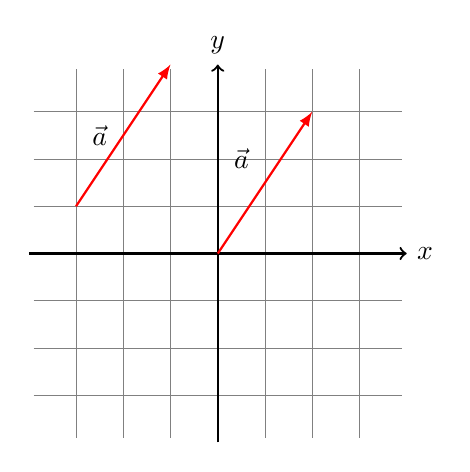
\begin{tikzpicture}[scale = 0.6]
    \draw[help lines, color=gray] (-3.9,-3.9) grid (3.9,3.9);
    \draw[->, thick] (-4,0)--(4,0) node[right]{$x$};
    \draw[->, thick] (0,-4)--(0,4) node[above]{$y$};

    \node[] at (0.5,2) {$\vec{a}$};
    \node[] at (-2.5,2.5) {$\vec{a}$};
    % \draw [fill=blue] (A) circle (2pt) node [left] {A};
    % \draw [fill=blue] (B) circle (2pt) node [left] {B};
    
    \draw [-latex, red, thick] (0, 0) -- (2, 3);
    \draw [-latex, red, thick] (-3, 1) -- (-1, 4);
  \end{tikzpicture}
\end{center}
I figuren ovanför så ser vi två lämpliga illustrationer av vektorn $\vec{a}$. Den ena börjar i origo
och har sin endpunkt vid (2, 3) och den andra börjar i (-3, 1) och slutar i (-1, 4). Man får alltså 
"flytta" runt sin vektor så länge riktingen och storleken (längden) blir oförändrade. 
\end{exmp}

%kanske en riktig definition här??
Addition och multiplikation av en skalär (slarvigt sagt en konstant) 
har också definerats.
För att addera två vektorer numeriskt så adderar 
man korresponderande komponenter med varandra. 
Låt exempelvis $\vec{a} = [-2, 5]$ och $\vec{b} = [6, 1]$, 
då är 
\[\vec{a} + \vec{b} = [-2 + 6, 5 + 1] = [4, 6].\]
För att multiplicera en skalär
med en vektor så multiplicerar man varje komponent med den skalären,
\[c \cdot \vec{a} = [-2 \cdot c, 5 \cdot c].\]
Det grafiska resultatet av dessa operationer lämnas som ett 
litet experiment till läsaren. 
Notera att vi kan subtrahera två vektorer genom att multiplicera den ena vektorn med 
$-1$ och sedan addera dem. 
% RITA KANSKE EN GRAF, BEROENDE PÅ OM JAG KOMMER HA PLATS MED DET!
% För en grafisk visualisering av addition och subtrahion så sätter man vektorerna i följd på varandra.
\begin{mydef}{}{}
  \textit{Skalärprodukten} mellan två vektorer $a$ och $b$ i $\mathbb{R}^n$ 
  betecknas $\langle \vec{a}, \vec{b} \rangle$ och ges av
  \[\langle \vec{a}, \vec{b} \rangle \equiv [a_1, a_2, \ldots, a_n] 
  \begin{bmatrix}
    b_1 \\
    b_2 \\
    \vdots \\
    b_n
  \end{bmatrix} = a_1 b_1 + a_2 b_2 + \ldots + a_n b_n.
  \]
\end{mydef}
Anledningen till varför den ena vektorn är horisontell och den andra vertikal är för att 
underlätta senare koncept. Båda vektorerna kan alltså vara horisontella eller vertikala 
om man så önksar. 
\begin{exmp}
  Betrakta vektorerna $\vec{a} = [-2, 5]$ och $\vec{b} = [6, 1]$. 
  Skalärprodukten av $\vec{a}$ och $\vec{b}$ ges då av
  \[\langle \vec{a}, \vec{b} \rangle = [-2, 5] 
\begin{bmatrix}
  6 \\
  1
\end{bmatrix} = -2 \cdot 6 + 5 \cdot 1 = -7.
\]  
\end{exmp}

Notera att skalärprodukten bara kan utföras på två vektorer om de har samma längd. 
Skalärprodukten mellan en vektorer i till exempel $\mathbb{R}^3$ och en annan vektor i $\mathbb{R}^2$
är alltså odefinerad eftersom det saknas korresponderande element. 

Eftersom skalärprodukten bara adderar produkter så blir resultatet alltid en skalär, vilket 
är förklaringen till namnet \textit{skalärprodukt}. 


\subsection{Matriser}
\begin{mydef}{}{}
  En $matris$ är ett rektangulärt schema av tal, symboler eller uttryck anordnade i rader och kolumner. 
  Dessa tal eller andra storheter i en matris kallas för \textit{element}.  
\end{mydef}
% -----------------------------------
%FLYTTA DELEN UNDER KOMMENTAREN LÄNGRE NER NÄR MAN HAR FÅTT EN INBLICK TILL VAD EN MATRIS ÄR.
% -----------------------------------
Viktigt att inse är att 
matriser inte är något naturligt matematiskt fenomen, 
utan ett sätt att lagra andra matematiska fenomen.
Till exempel så kan matriser vara användbara vid programering eller datorgrafik för att lagra data som 
pixlar på en skärm eller liknande. Vi ser också att vektorer egentligen bara är ett specialfall av en 
matris.
\begin{exmp}
Matrisen
\[ \underset{2 \times 3}{A} = 
  \begin{bmatrix}
    1 & 2 & 3 \\
    x & y & z
  \end{bmatrix}
\]
är en $2 \times 3$ matris och har alltså två rader och tre columner.
I denna matris så är $1, 2, 3, x, y$ och $z$ element i $\underset{2 \times 3}{A}.$
Det är inte nödvändigt att ange dimensionerna nedanför variablen, det är valfritt. 

För att uttrycka ett element i denna matris så anger man i vilket rad och kolumn 
elementet befinner sig i som ett nedre index. Till exempel så är 
$A_{21} = x$ och $A_{13} = 3$.
\end{exmp}

Operationer på matriser har också definerats. För att addera två matriser så adderar man helt enkelt korresponderande element med varandra. 
Låt exempelvis 
\[ A = 
  \begin{bmatrix}
    7 & -2 & 13 \\
    4 & 0 & 9
  \end{bmatrix}, \;
  B = 
  \begin{bmatrix}
    1 & 6 & -2 \\
    6 & 10 & 2
  \end{bmatrix}.
\]

Då är 
\begin{align*}
  A + B & =
  \begin{bmatrix}
    7 + 1 & -2 + 6 & 13 + (-2) \\
    4 + 6 & 0 + 10 & 9 + 2
  \end{bmatrix} \\
  & = 
  \begin{bmatrix}
    8 & 4 & 11 \\
    10 & 10 & 11
  \end{bmatrix}.
\end{align*}
För kunna addera två matriser så måste de alltså ha samma 
dimensioner. Till exempel så går det inte att 
addera $\underset{3 \times 1}{A}$ med $\underset{4 \times 4}{B}$ eftersom vissa element i den ena matrisen saknar ett korresponderande element i den andra matrisen.

För att multiplicera en skalär med en matris så multiplicerar man 
alla element i matrisen med den skalären. Vi låter $A$ vara samma matris som förut och $c$ en skalär.
Då är 
\[
c \cdot A = 
  \begin{bmatrix}
    7 \cdot c & -2 \cdot c & 13 \cdot c \\
    4 \cdot c & 0 \cdot c & 9 \cdot c
  \end{bmatrix}.
\]
För att multiplicera två matriser med varandra så blir det lite jobbigare. 
Istället för att definera multiplikation på liknande sätt som addition så har man valt att defiinera det lite annorlunda. Det har helt enkelt visat sig vara väldigt praktiskt med just
denna definition.

Vi väljer två "slumpmässiga" matriser $A$ och $B$, säg
\[
A = \begin{bmatrix}
  3 & 1 & 2 \\
  -1 & 0 & 5
\end{bmatrix}, \; 
B = 
\begin{bmatrix}
  -1 & 3 \\
  2 & 5 \\
  6 & 7
\end{bmatrix},
\]
och multiplicerar dem med varandra
\[A \times B = 
  \left[ 
  \;
  \begin{array}{cccc}
    \rowcolor{blue!20}
    3 & 1 & 2 \\
    \rowcolor{red!20}
    -1 & 0 & 5
  \end{array}
  \;
  \right]
  \left[
  \;
  \begin{array}{>{\columncolor{green!20}}c>{\columncolor{orange!40}}cc}
    1 & 3 \\
    2 & 5 \\
    6 & 7
  \end{array}
  \;
  \right].
\]
För att göra det enklare för oss så färglägger vi alla rader i $A$ och alla kolumner i $B$ med olika 
färger. Vi kan tänka oss att de färgglada områderna representerar vektorer. Vi namnger nu dessa 
"vektorer"/områden
baserat på vilken färg de har, \textcolor{blue!60}{$B$}
för det blåa området, \textcolor{red!60}{$R$} för det röda, \textcolor{green!70!black}{$G$} för det gröna och 
\textcolor{orange!60}{$O$} för det orangea. Definitionen av matris multiplikation lyder att 
\[A \times B = 
\begin{bmatrix}
  \langle \textcolor{blue!60}{B}, \textcolor{green!70!black}{G} \rangle &
  \langle \textcolor{blue!60}{B}, \textcolor{orange!60}{O} \rangle \\
  \langle \textcolor{red!60}{R}, \textcolor{green!70!black}{G} \rangle &
  \langle \textcolor{red!60}{R}, \textcolor{orange!60}{O} \rangle
\end{bmatrix}.
\]
För att få fram några vettiga element för $A \times B$ så måste vi utföra dessa skalärprodukter. 
\begin{align*}
  \langle \textcolor{blue!60}{B}, \textcolor{green!70!black}{G} \rangle &= 
  3 \cdot 1 + 1 \cdot 2 + 2 \cdot 6 = 17,\\
  \langle \textcolor{blue!60}{B}, \textcolor{orange!60}{O} \rangle &= 
  3 \cdot 3 + 1 \cdot 5 + 2 \cdot 7 = 28, \\
  \langle \textcolor{red!60}{R}, \textcolor{green!70!black}{G} \rangle &=
  -1 \cdot 1 + 0 \cdot 2 + 5 \cdot 6 = 29, \\
  \langle \textcolor{red!60}{R}, \textcolor{orange!60}{O} \rangle &=
  -1 \cdot 3 + 0 \cdot 5 + 5 \cdot 7 = 32,
\end{align*}
och därför blir 
\[A \times B =
\begin{bmatrix}
  17 & 28 \\
  29 & 32
\end{bmatrix}.
\]
Vi ser att multiplikation av två matriser endast kan ske om den första matrisen har lika många kolumner
som den andra har rader. Till exempel så kan man multiplicera $\underset{2 \times 3}{A}$ med 
$\underset{3\times 2}{B}$ men inte $\underset{2 \times 4}{A}$ med $\underset{3 \times 3}{B}$ eftersom 
skalärprodukten bara kan utföras på två vektorer om de har samma längd.

För att bevisa att multiplikation av matriser inte är kommutativ så kan man 
beräkna $B \times A$ och jämföra resultatet med $A \times B$. Detta lämnas som en övning till läsaren.

\begin{mydef}{Identitetsmatrisen}{}
  \textit{Identitetsmatrisen} är en $n \times n$ matris som har ettor längst diagonalen (från övre vänstra 
  till nedre högra hörnet) och nollor överallt annars och betecknas med $I_n,$
  \[\underset{n \times n}{I_n} =
  \left[
  \;
  \begin{array}{>{\columncolor{green!20}}c>{\columncolor{orange!40}}cc
    >{\columncolor{blue!20}}c}
    1 & 0 & \cdots & 0 \\
    0 & 1 & \cdots & 0 \\
    \vdots & \vdots & \ddots & \vdots \\
    0 & 0 & \cdots & 1
  \end{array}
  \;
  \right].
  \]
  Varje kolumn i identitetsmatrisen har fått en beteckning, det gröna området 
  betecknas med $\vec{e}_1$, det orangea med $\vec{e}_2$ och det blåa med $\vec{e}_n.$ Notera att 
  $I_n = [\vec{e}_1, \vec{e}_2, \ldots, \vec{e}_n].$
\end{mydef}

\begin{exmp}
  Matrisen 
  \[
  \begin{bmatrix}
    1 & 0 & 0 \\
    0 & 1 & 0 \\
    0 & 0 & 1
  \end{bmatrix}
  \]
  är identitetsmatrisen $I_3$ och består av 
  \[ \vec{e}_1 = 
  \begin{bmatrix}
    1 \\
    0 \\
    0
  \end{bmatrix}, 
  \vec{e}_2 = 
  \begin{bmatrix}
    0 \\
    1 \\
    0
  \end{bmatrix},
  \vec{e}_3 = 
  \begin{bmatrix}
    0 \\
    0 \\
    1
  \end{bmatrix}
  \]
  och därför är $I_3 = [\vec{e}_1, \vec{e}_2, \vec{e}_3].$
\end{exmp}

En viktig egenskap hos identitetsmatriserna är att 
\[\underset{m \times n}{A} I_n = \underset{m \times n}{A} = I_m \underset{m \times n}{A}\]
vilket enkelt kan visas genom att multiplicera matriserna. 



\subsection{Linjära transformationer}
En \textit{transformation} är egentligen bara en funktion. Man ger funktionen en mängd och funktionen 
mappar alla element med ett korresponderande element från en annan mängd. I linjär algebra brukar man 
dock tänka att en transformation mappar en vektor med en annan vektor. Anledningen till namnet 
\textit{transformation} och inte \textit{funktion} sitter i visualiseringen. Man kan tänka att en 
transformation "gör om", eller transformerar, 
en vektor till en annan vektor genom att till exempel rotera den, göra 
den längre eller liknande. En transformation brukar betecknas med ett $T$. 

\begin{exmp}
  Betrakta transformationen $T: \mathbb{R}^3 \rightarrow \mathbb{R}^2$ som defineras av 
\[T \left(
  \begin{bmatrix}
    x_1 \\
    x_2 \\
    x_3
  \end{bmatrix}
\right) = 
\begin{bmatrix}
  x_1 + x_2 \\
  x_3 x_2 
\end{bmatrix}.
\]
För att kolla vad denna transformation gör med en vektor 
så kan vi välja en slumpmässig vektor i $\mathbb{R}^3$, säg
\[\vec{v} = 
\begin{bmatrix}
  1 \\
  2 \\
  1
\end{bmatrix}
\]
och sedan kolla på vad $T(\vec{v})$ blir. 
\[T(\vec{v}) = 
\begin{bmatrix}
  1 + 2 \\
  1 \cdot 2
\end{bmatrix} = 
\begin{bmatrix}
  3 \\
  2
\end{bmatrix}.
\]

\begin{center}
  \begin{tikzpicture}
    \draw (0,0,0) --  (2,0,0)  node[pos=1.05]{$x$};
    \draw (0,0,0) -- (0,3,0) node[pos=1.05]{$y$};
    \draw (0,0,0) -- (0,0,2) node[pos=1.1]{$z$};

    \draw [-latex, red, thick] (0, 0, 0) -- (1, 2, 1);
    \draw[dashed, red, thick] (0, 0, 0) -- (1, 0, 1);
    \draw[dashed, red, thick] (1, 0, 1) -- (1, 2, 1);
    \node[scale = 1] at (1, 2.3, 1) {$(1, 2, 1)$};

    \draw [-latex] (2.7, 1, 0) -- (4.3, 1, 0);
    \node at (3.5, 1.5, 0) {$T(\vec{v})$};

    \draw (5, 0) -- (7, 0) node[pos=1.05] {$x$};
    \draw (5, 0) -- (5, 2) node[pos=1.05] {$y$};
    \draw [-latex, red] (5, 0) -- (6.5, 1);
    \node at (6.5, 1.4) {$(3, 2)$};
  \end{tikzpicture}
\end{center}
I figuren ovan ser vi visuellt hur vektorn $v$ transformeras av $T$. 
\end{exmp}

En \textit{linjär} transformation är inget mer än en vanlig transformation som måste uppfylla två villkor. 

\hypertarget{linjarT}{}
\begin{mydef}{Linjär transformation}{}
  En \textit{linjär transformation} mellan $\mathbb{R}^n$ och $\mathbb{R}^m$ (mer generellt
  mellan två vektorrum) är en transformation $T: \mathbb{R}^n \rightarrow \mathbb{R}^m$
  där följande villkor uppfylls
  \begin{enumerate}[I.]
    \item $T(\vec{v_1} + \vec{v_2}) = T(\vec{v_1}) + T(\vec{v_2}),$
    \item $cT(\vec{v_1}) = T(c \vec{v_1}),$
  \end{enumerate}
  för två vektorer $\vec{v_1}, \vec{v_2}$ 
     i $\mathbb{R}^n$ och en skalär $c.$
\end{mydef}
Med hjälp av linjära transformationer så kan vi ställa upp följande sats som blir användbar senare. 

\hypertarget{linjarTsats}{}
\begin{mytheo}{}{}
  En linjär transformation $T: \mathbb{R}^n \rightarrow \mathbb{R}^m$ kan representeras 
  som 
  \[T(\vec{v}) = [ \; T(\vec{e}_1), \; T(\vec{e}_2), \ldots, \; T(\vec{e}_n) \;] \vec{v}\]
  för en vektor $\vec{v} \in \mathbb{R}^n$ och där $\vec{e}_1, \vec{e}_2, \ldots, \vec{e}_n \in I_n$
\end{mytheo}
\begin{proof}
  Låt $\vec{v}$ vara en vektor i $\mathbb{R}^n$ definerad som
  \[\vec{v} = 
  \begin{bmatrix}
    v_1 \\
    v_2 \\
    \vdots \\
    v_n
  \end{bmatrix},
  \]
  då gäller det att 
  \[
    v = I_n v = [\vec{e}_1, \; \vec{e}_2, \ldots, \; \vec{e}_n] 
    \begin{bmatrix}
      v_1 \\
      v_2 \\
      \vdots \\
      v_n
    \end{bmatrix} = \vec{e}_1 v_1 + \vec{e}_2 v_2 + \cdots + \vec{e}_n v_n 
  \]
  \[\iff\]
  \[
    T(v) = T(\vec{e}_1 v_1 + \vec{e}_2 v_2 + \cdots + \vec{e}_n v_n).
  \]
    Eftersom $T$ är en linjär transformation så måste den uppfylla villkoren I och II enligt
  \hyperlink{linjarT}{definition 3.4.1}. Vid användning av I får vi 
  \[T(v) = T(\vec{e}_1 v_1) + T(\vec{e}_2 v_2) + \cdots + T(\vec{e}_n v_n)\]
  och sedan av II
  \begin{align*}
    T(v) &= v_1 T(\vec{e}_1) + v_2 T(\vec{e}_2) + \cdots + v_n T(\vec{e}_n) \\
    &= [ \; T(\vec{e}_1) +  T(\vec{e}_2) + \cdots +  T(\vec{e}_n) \;]
    \begin{bmatrix}
      v_1 \\
      v_2 \\
      \vdots \\
      v_n
    \end{bmatrix} \\
    &=  [ \; T(\vec{e}_1) +  T(\vec{e}_2) + \cdots +  T(\vec{e}_n) \;] \vec{v}.
  \end{align*}
\end{proof}


%kanske bättre att ha med \textbf{exempel 3.1} blablalbla. 


\subsubsection{Rotationer i \texorpdfstring{$\mathbb{R}$$^3$}{}}
Detta avsnitt kommer att kolla på en speciell linjär transformation, nämligen en rotation
kring $x, y$ och $z-$axeln. Beviset av att en rotation är en linjär transformation är inte 
särskilt interesant och inte heller elegant, så det kommer att utelämnas i denna text. Vi får 
helt enkelt ta det som givet för denna stund. 

För att beteckna en rotation moturs med $\theta$ 
kommer $Rot_{x\theta}$, $Rot_{y\theta}$ och $Rot_{z\theta}$ användas för att indikera vilken 
axel vi roterar krign.
Vi börjar med att ställa upp följande sats

\begin{mytheo}{}{}
  En moturs rotation $Rot_{n\theta} : \mathbb{R}^3 \rightarrow \mathbb{R}^3, \; n \in \{x, y, z\}$ 
  med $\theta$ i $\mathbb{R}^3$ av en vektor $\vec{v} \in \mathbb{R}^3$ ges av 
  \begin{align}
    Rot_{x\theta} (\vec{v}) &= 
    \begin{bmatrix}
      1 & 0 & 0 \\
      0 & \cos(\theta) & -\sin(\theta) \\
      0 & \sin(\theta) & \cos(\theta)
    \end{bmatrix} \vec{v}, \\
    Rot_{y\theta} (\vec{v}) &= 
    \begin{bmatrix}
      \cos(\theta) & 0 & \sin(\theta) \\
      0 & 1 & 0 \\
      -\sin(\theta) & 0 & \cos(\theta)
    \end{bmatrix} \vec{v}, \\
    Rot_{z\theta} (\vec{v}) &= 
    \begin{bmatrix}
      \cos(\theta) & -\sin(\theta) & 0 \\
      \sin(\theta) & \cos(\theta) & 0 \\
      0 & 0 & 1
    \end{bmatrix} \vec{v}.
  \end{align}
\end{mytheo}

\begin{proof}
  Vi visar först att (1) gäller innan vi går vidare. Låt $\vec{v}$ vara en vektor i $\mathbb{R}^3$. 
  Eftersom en rotation är en linjär transformation så gäller \hyperlink{linjarTsats}{sats 3.4.1} och 
  därför är
  \[Rot_{x\theta} (\vec{v}) = [\; Rot_{x\theta} (\vec{e}_1), Rot_{x\theta} (\vec{e}_2), 
  Rot_{x\theta} (\vec{e}_3)\;] \vec{v}\]
  där $\vec{e}_1, \vec{e}_2, \vec{e}_3 \in I_3.$
  Vi skall alltså analysera hur $\vec{e}_1 = 
  \begin{bmatrix}
    1 \\
    0 \\
    0
  \end{bmatrix}
  , \vec{e}_2 = 
  \begin{bmatrix}
    0 \\
    1 \\
    0
  \end{bmatrix}
  , \vec{e}_3 = 
  \begin{bmatrix}
    0 \\
    0\\
    1
  \end{bmatrix}
  $ förändras efter en rotaion med 
  $\theta$ kring $x-$axeln och till våran hjälp har vi figuren nedanför. 

  \newcommand{\AxisRotator}[1][rotate=0]{%
    \tikz [x=0.2cm,y=0.60cm,line width=.2ex,-stealth,#1] \draw (0,0) arc (-150:150:1 and 1);%
  }

  \begin{center}
    \begin{tikzpicture}
      \draw (0,0,0) --  (2,0,0)  node[pos=1.05]{$x$};
      \draw (0,0,0) -- (0,2,0) node[pos=1.05]{$y$};
      \draw (0,0,0) -- (0,0,2) node[pos=1.1]{$z$};
      \draw (0,0)  -- (1.8,0)  node [near end, scale=0.5] {\AxisRotator};
      
      \draw[thick, ->] (0,0,0) -- (1,0,0) node at (0.6, 0.3){$\vec{e_1}$};
      \draw[thick, ->] (0,0,0) -- (0,1,0) node at (-0.3, 0.6){$\vec{e_2}$};
      \draw[thick, ->] (0,0,0) -- (0,0,1) node at (-0.2, -0.6){$\vec{e_3}$};
      \node at (1, -0.3, 0) {1};
      \node at (0.3, 1, 0) {1};
      \node at (-0.3, 0, 1) {1};
    \end{tikzpicture}
  \end{center}
  $\vec{e}_1$ kommer att vara oförändrad efter en rotation kring $x-$axeln, 
  \[Rot_{x\theta}(\vec{e}_1) = 
  \begin{bmatrix}
    1 \\
    0 \\
    0
  \end{bmatrix}
  .\]
  Vi kollar närmare på hur $\vec{e}_1$ och $\vec{e}_2$ förändras efter en rotation. 
  \begin{center}
    \begin{tikzpicture}
      \draw (0,-2) -- (0,2) node[pos=1.05]{$y$};
      \draw (2,0) -- (-2,0)  node[pos=1.05]{$z$};

      \draw[thick, ->] (0,0) -- (-1,1) node at (-1.3, 1.3){$\vec{e}_2$};
      \draw[thick, dashed] (0,1) -- (-1,1);
      \draw[thick, dashed, white] (0,0) -- (0,1);
      \coordinate (a) at (0, 2);
      \coordinate (b) at (0, 0);
      \coordinate (c) at (-1, 1);
      \pic [draw, ->, "$\theta$", angle eccentricity=1.5] {angle = a--b--c};

      \draw[thick, ->] (0,0) -- (-1,-1) node at (-1.3, -1.3){$\vec{e}_3$};
      \draw[thick, dashed] (-1,0) -- (-1,-1);
      \draw[thick, dashed, white] (0,0) -- (-1,0);
      \coordinate (a) at (-2, 0);
      \coordinate (b) at (0, 0);
      \coordinate (c) at (-1, -1);
      \pic [draw, ->, "$\theta$", angle eccentricity=1.5] {angle = a--b--c};
    \end{tikzpicture}
  \end{center}
  $x-$komponanten för $\vec{e}_2$ och $\vec{e}_3$ är fortfarande noll eftersom de ligger på $y-$axeln. 
  Med enkel trigonometri så ser vi att $y-$komponanten för $\vec{e}_2$ är $\cos(\theta)$ och att 
  $z-$komponanten är $\sin(\theta)$ och därför är 
  \[Rot_{x\theta} (\vec{e}_2) = 
  \begin{bmatrix}
    0 \\
    \cos(\theta) \\
    \sin(\theta) 
  \end{bmatrix}.
  \] 
  Samma princip gäller för $\vec{e}_3$ och vi får att 
  \[Rot_{x\theta} (\vec{e}_3) = 
  \begin{bmatrix}
    0 \\
    -\sin(\theta) \\
    \cos(\theta)
  \end{bmatrix},
  \]
  vilket betyder att 
  \begin{align*}
    Rot_{x\theta} (\vec{v}) &= [\; Rot_{x\theta} (\vec{e}_1), Rot_{x\theta} (\vec{e}_2), 
    Rot_{x\theta} (\vec{e}_3)\;] \vec{v} \\
    &=
    \begin{bmatrix}
      1 & 0 & 0 \\
      0 & \cos(\theta) & -\sin(\theta) \\
      0 & \sin(\theta) & \cos(\theta)
    \end{bmatrix} \vec{v}.
  \end{align*}
  För 
  $Rot_{y\theta} (\vec{v})$ gäller det att 
  \[Rot_{y\theta} (\vec{v}) = [\; Rot_{y\theta} (\vec{e}_1), Rot_{y\theta} (\vec{e}_2), 
  Rot_{y\theta} (\vec{e}_3)\;] \vec{v}.\]
  $\vec{e}_2$ ligger på $y-$axeln och blir därför inte påverkad av en rotation.
  \[Rot_{y\theta} (\vec{e}_2) = 
  \begin{bmatrix}
    0 \\
    1 \\
    0
  \end{bmatrix}.
  \]
  Med trigonometri får vi även att 
  \[Rot_{y\theta} (\vec{e}_1) = 
  \begin{bmatrix}
    \cos(\theta) \\
    0 \\
    -\sin(\theta)
  \end{bmatrix}, \; Rot_{y\theta} (\vec{e}_3) = 
  \begin{bmatrix}
    \sin(\theta) \\
    0 \\
    \cos(\theta)
  \end{bmatrix}
  \]
  vilket betyder att 
  \[Rot_{y\theta} (\vec{v}) = 
  \begin{bmatrix}
    \cos(\theta) & 0 & \sin(\theta) \\
    0 & 1 & 0 \\
    -\sin(\theta) & 0 & \cos(\theta)
  \end{bmatrix} \vec{v}.\]
  För att visa att (3) gäller så använder man precis samma strategi. Denna del lämnas 
  som en övning till läsaren.
\end{proof}

\begin{exmp}
  Låt $\vec{v} = \begin{bmatrix}
    0 \\
    1 \\
    0
  \end{bmatrix}.$
  $Rot_{x \pi/2} (\vec{v})$ defineras då som
  \begin{align*}
    Rot_{x \pi/2} (\vec{v}) &= 
    \begin{bmatrix}
        1 & 0 & 0 \\
        0 & \cos(\frac{\pi}{2}) & -\sin(\frac{\pi}{2}) \\
        0 & \sin(\frac{\pi}{2}) & \cos(\frac{\pi}{2})
    \end{bmatrix}
    \begin{bmatrix}
      0 \\
      1 \\
      0
    \end{bmatrix} \\
    &= \begin{bmatrix}
      0 \\
      0 \\
      1
    \end{bmatrix}
  \end{align*}
  och roterar alltså $\vec{v}$ 90 grader moturs som bilden nedan illustrerar.
  %ta kanske bort denna bild, tar upp mycket plats?? Eller?????????
  \begin{center}
    \begin{tikzpicture}
      \draw (0,0,0) --  (2,0,0)  node[pos=1.05]{$x$};
      \draw (0,0,0) -- (0,2,0) node[pos=1.05]{$y$};
      \draw (0,0,0) -- (0,0,2) node[pos=1.1]{$z$};
      \draw [-latex, thick] (0, 0, 0) -- (0, 1, 0) node at (0.4, 1) {$\vec{v}$};
      \draw [-latex, thick] (0, 0, 0) -- (0, 0, 1) node at (0.7, -0.5) {$Rot_{x \pi/2} (\vec{v})$};
    \end{tikzpicture}
  \end{center}
\end{exmp}

\section{Gruppteori}
%---------------VIKTIGT------------------
%ändra introduktionen till gruppteori. Säg att addition kommer att användas occaisonaly 
%när det är nödvändigt men att vi kommer att diskutera det i djupet senare. 
Gruppteori är en väldig central del inom abstrakt algebra. 
Inom den abstrakta algebran så studerar man olika algebraiska strukturer
såsom grupper, ringar, kroppar och liknande strukturer och skiljer sig därmed från den elementära algebran. 

Man kan inom viss mån säga att den elementära algebran studerar de 
vanligaste talsystemen, $\mathbb{N}, \; \mathbb{Z}, \; \mathbb{Q}, \; \mathbb{R}, \; \mathbb{C}$,
och användingen av dessa.
Den elementära algebran är på så sätt 
extremt kraftfull. Det är exempelvis alltid användbart att kunna addera, subtrahera och 
ställa upp ekvationer 
med reella tal eftersom vi alltid kan dra parrallerer mellan dem
och den verkliga världen. Detta är också anledningen till varför den elementära algebran
studeras så mycket. 

Den abstrakta algebran står lite på andra ändan av snörret när det gäller 
talsystem. Istället för att anaysera användningarna av de vanligaste talsystemen så 
ställs istället frågan om man kan hitta på nya och interesanta talsystem. Hela målet med detta är att försöka klämma ut vissa egenskaper hos de vanligaste 
talsystemen för att på så sätt generalisera det vi menar med ett användbart talsystem.

Det är möjligt att abstrahera bort praktiskt taget alla egenskaper hos ett talsystem för att skapa en struktur som kallas för en magma. Problemet med detta är att en
magma är alldeles för generell för att vara intresann. På samma sätt kan man abstrahera bort praktiskt taget inga egenskaper för att hitta
många resultat men som samtidigt blir alldeles för specifik för att lösa generella problem. Man vill alltså hitta en balans mellan dessa två extremfall och det man blir kvar med då är grupper och 
ringar. Ibland används även dessa extremfall ändå, till exempel så används monoider i datavetenskap vid användning av abstrakta datatyper. 

Denna text får tyvärr inte plats med alla dessa interesanta algebraiska strukturer. I slutet va denna text kommer vi dock att hänvisa till andra fantastiska källor där man
kan lära sig mycket om abstrakt algebra och även häftiga tillämpningar av grupper. I denna text kommer vi alltså att ägna åt oss grupper. 

Gruppteori är inte bara användbart för att generalisera vissa talsystem, utan används även som en abstrakt \textit{notation} för symmetri (vanligtvisst brukar man 
missförstå grupper och säga att de beskriver symmetrier av ett givet \textit{objekt}. Detta kallas dock för gruppverkan, vilket är ett sätt att tillämpa notationer för symmetri på ett givet objekt).
Detta gör att grupper blir tillämpliga i många olika området, allt från relationer mellan polynom och dess röter (Galois teori) coh lösningarna av en Rubiks kub.

Innan vi börjar våran abstrakta grupp resa så kollar vi på följande talsystem
\[ \mathbb{Z} = \{0, 1, -1, 2, -2, \ldots\}. \]
Det som gör detta talsystem mycket mer än en tråkig mängd med symboler är att 
vi har ett sätt att \textit{sammansätta} två element. Man kan till exempel 
addera 1 med 2 för att få 3, men vad menas det egentligen med att "addera" två heltal? Vad står 1 och 2 för? Det kan kännas som en dum fråga, men det finns faktiskt ett sätt 
att förstå addition och heltal på med hjälp av grupper. Men innan vi går igenom detta så inför vi en ny beteckning, $\circ$, för "sammansättning". Denna "sammansättning" kommer 
att fungera som en operation som man kan \textit{definera hur man än vill}. Detta gör att vi inte behöver begränsa oss till endast addition för att generelisera grupper lite mer. 
Senare i texten kommer vi att dedikera denna symbol till en specifik operation för att underlätta saker och ting. 

Med detta ur vägen så kan vi nu definera vad en grupp är. 

\hypertarget{def4.1}{}
\begin{mydef}{Grupp}{}
  En \textit{grupp} $G$ under operationen $\circ$, vilket skrivs $(G, \circ)$,
  är en mängd som uppfyller följande \textit{grupp axiom}
  \begin{enumerate}[I)] 
    \item \textbf{Slutenhet.} $x \circ y \in G, \; \forall x, y \in G.$ 
    \item \textbf{Assosiativitet.} $(x \circ y) \circ z = x \circ (y \circ z), \; \forall x, y \in G.$
    \item \textbf{Enhetselementet.} $\exists! e \in G \; | \; x \circ e = e \circ x = x.$
    \item \textbf{Inverser.} $\forall x \in G, \exists ! x^{-1} \in G \; | \; x \circ x^{-1}
    = x^{-1} \circ x = e,$
  \end{enumerate}
  där $\exists !$ betyder att det existerar exakt ett. Kardinaliteten av $G$ kallas 
  för \textit{ordningen} och betecknades $|G|$.
\end{mydef}

\begin{exmp}
  Heltalen under addition, $(\mathbb{Z}, +)$, skapar en grupp eftersom grupp axiomen 
  \textbf{sluthet, assosiativitet, enhetselementet} och \textbf{inverser} uppfylls.

  \begin{enumerate}[I)]
    \item \textbf{Slutenhet.} För alla heltal $x$ och $y$ så är alltid $x + y$ ett heltal. 
    \item \textbf{Assosiativitet.} För alla heltal $x, y, z$ så gäller $(x + y) + z = x + (y + z).$
    \item \textbf{Enhetselementet.} Enhetselementet är 0 eftersom $x + 0 = 0 + x = x,$ för alla heltal $x.$
    \item \textbf{Inverser.} Inversen för ett heltal $x$ är $-x$ eftersom $x + (-x) = (-x) + x = 0.$
  \end{enumerate}
\end{exmp}
Notera att grupp axiomen inte nämner något om kommutativitet. Det kan allså gälla att 
$x \circ y = y \circ x$ men detta är inte nödvändigt. För att särskilja sådana grupper från 
varandra så gör vi följande definition.
\begin{mydef}{Abelsk grupp}{}
  En \textit{abelsk grupp} $G$ är kommutativ, $x \circ y = y \circ x, \forall x, y \in G.$
\end{mydef}

\subsection{Konstruktion av en grupp}
För att konstruera en unik grupp så måste man först skapa en mängd av symboler och definera 
en operation på elementen så att alla grupp axiom uppfylls.
Som man kanske kunde gissat sig fram så blir detta svårt om vi vill skapa något nytt 
utan att använda de vanliga räknesätten. För att göra det enklare så görs följande definition.
\begin{mydef}{Permutation}{}
  En \textit{permutation} är en bijektion från en mängd till sig själv. En grupp innehållande 
  permutationer kallas för en \textit{permutationsgrupp}.
\end{mydef}
%definera vad en permutationsgrupp är här uppe.
Det blir betydligt mycket lättare att konstruera en unik grupp genom att använda permutationer. 
Man kan nämligen tänka sig att en grupp innehåller olika permutationer av en annan mängd. 

För att konstruera våran första grupp så skapar vi mängden $S = \{a, b\}.$
Alla möjliga permutationer av $S$ är 
\begin{center}
  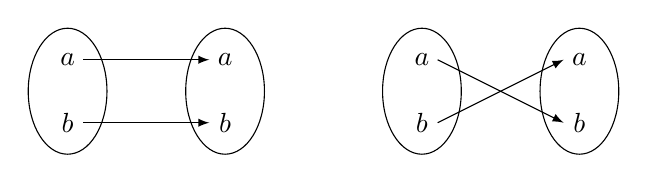
\begin{tikzpicture}
    \draw (0,0) ellipse (0.5cm and 0.8cm);
    \node at (0, 0.4) {$a$};
    \node at (0, -0.4) {$b$};
    \draw (2,0) ellipse (0.5cm and 0.8cm);
    \node at (2, 0.4) {$a$};
    \node at (2, -0.4) {$b$};

    \draw[-latex] (0.2, 0.4) -- (1.8, 0.4);
    \draw[-latex] (0.2, -0.4) -- (1.8, -0.4);

    \draw (4.5,0) ellipse (0.5cm and 0.8cm);
    \node at (4.5, 0.4) {$a$};
    \node at (4.5, -0.4) {$b$};
    \draw (6.5,0) ellipse (0.5cm and 0.8cm);
    \node at (6.5, 0.4) {$a$};
    \node at (6.5, -0.4) {$b$};

    \draw[-latex] (4.7, 0.4) -- (6.3, -0.4);
    \draw[-latex] (4.7, -0.4) -- (6.3, 0.4);
  \end{tikzpicture}
\end{center}
Vi kan nu beteckna dessa permutationer beroende på hur elementen "byter plats". Permutationen
till vänster mappar $a$ till $a$ och $b$ till $b$ och agerar som ett enhetselement. En 
logisk beteckning för denna är därför $e$. Permutationen till höger mappar $a$ till $b$ och 
$b$ till $a$ och en vanlig beteckning för detta är $\tau.$ 
Med hjälp av Cauchy notationen så kan vi skriva dessa permutationer som 
\[e = 
\begin{pmatrix}
  a & b \\
  a & b
\end{pmatrix},
\tau = 
\begin{pmatrix}
  a & b \\
  b & a
\end{pmatrix}.
\]
Denna notation använder sig av en matris där den första raden anger elementen av en mängd 
och vad elementen blir mappade till i den andra raden.
Till exempel så är $\tau (a) = b, \; e(b) = b.$
Vi kan nu skapa en ny mängd
$G$ som innehåller dessa permutationer på följande sätt.
\[G = \{e, \tau\}.\]
Operationen $\circ$ kan nu defineras som den resulterande permutationen efter att ha 
tillämpat två permutationer efter varandra, $f \circ g = f(g), \; f, g \in G.$ Denna operation kallas för \textit{komposition} och används på många andra ställen i matematiken också.
Exempelvis så är $\tau \circ e = 
\tau (e)$ och genom att kolla på figuren nedan så kan vi dra slutsatsen att 
$\tau (e) = \tau$ och att $\tau (e(a)) = b.$ 

\begin{center}
  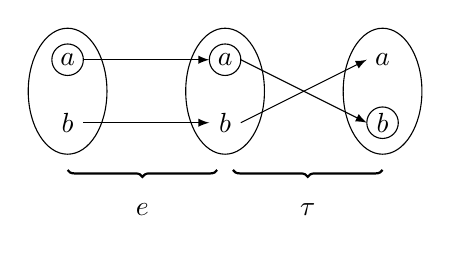
\begin{tikzpicture}
    \draw (0,0) ellipse (0.5cm and 0.8cm);
    \node at (0, 0.4) {$a$};
    \draw (0,0.4) ellipse (0.2cm and 0.2cm);
    \node at (0, -0.4) {$b$};
    \draw (2,0) ellipse (0.5cm and 0.8cm);
    \draw (2,0.4) ellipse (0.2cm and 0.2cm);
    \node at (2, 0.4) {$a$};
    \node at (2, -0.4) {$b$};

    \draw[-latex] (0.2, 0.4) -- (1.8, 0.4);
    \draw[-latex] (0.2, -0.4) -- (1.8, -0.4);

    % \draw[-latex] (2.2, 0.4) -- (4.3, 0.4);
    % \draw[-latex] (2.2, -0.4) -- (4.3, -0.4);

    % \draw (4.5,0) ellipse (0.5cm and 0.8cm);
    % \node at (4.5, 0.4) {$a$};
    % \draw (4.5,0.4) ellipse (0.2cm and 0.2cm);
    % \node at (4.5, -0.4) {$b$};
    \draw (4,0) ellipse (0.5cm and 0.8cm);
    \node at (4, 0.4) {$a$};
    \node at (4, -0.4) {$b$};
    \draw (4,-0.4) ellipse (0.2cm and 0.2cm);

    \draw[-latex] (2.2, 0.4) -- (3.8, -0.4);
    \draw[-latex] (2.2, -0.4) -- (3.8, 0.4);

    \draw [
    thick,
    decoration={
        brace,
        mirror,
        raise=0.5cm
    },
    decorate
] (0, -0.5) -- (1.9, -0.5) node [pos=0.5, yshift = -1cm] {$e$}; 

\draw [
  thick,
  decoration={
      brace,
      mirror,
      raise=0.5cm
  },
  decorate
] (2.1, -0.5) -- (4, -0.5) node [pos=0.5, yshift = -1cm] {$\tau$}; 
  \end{tikzpicture}
\end{center}

Notera att man först behöver utföra $e(a)$ innan $\tau (e(a))$.
På grund av detta 
så kommer $f \circ g, \; f, g \in G$ betyda att vi utför permutationen $g$ först 
och sedan $f$ och \textbf{inte} tvärtom. 

%skriv vad tabellen heter.
Vi kan nu skapa en tabell likt en multiplikations tabell som visar alla möjliga 
permutations sammansättningar av $G$. Detta kallas för en \textit{Cayles tabell} och kan användas för att definera operationen $\circ$.

\begin{minipage}{\textwidth}
\centering
  \begin{tabular}{c | c c}
    $\circ$ & $e$ & $\tau$ \\
    \cline{1-3}
    $e$ & $e$  &$\tau$ \\
    $\tau$ & $\tau$  &$e$\\
  \end{tabular} 

  \medskip
  \footnotesize
  Tabell 1.
\end{minipage}

Elementen i $G$ är inte längre några tråkiga symboler utan något betydligt mer, nämligen permutationer. 
Vi har även ett sätt att sammansätta två permutationer, precis som man kan sammansätta två element
i $\mathbb{Z}.$ Dessutom så har permutationer en väldigt användbar egenskap som följande sats 
tar upp. 
\hypertarget{ass}{}
\begin{mytheo}{}{}
  Permutationer är associativa,
  \[(f \circ g) \circ h(x) = f \circ (g \circ h(x))\]
  för tre permutationer $f, g$ och $h$ från mängden $X$ till $X$ där $x \in X.$
\end{mytheo}
\begin{proof}
  Vänster ledet ger oss 
  \[V.L = (f \circ g) \circ h(x) = f(g(h(x)))\]
  och höger ledet ger 
  \[H.L = f \circ (g \circ h(x)) = f \circ g(h(x)) = f(g(h(x))).\]
  $V.L = H.L$ och beviset är slutfört.
\end{proof}

Det som återstår är att visa är att $G$ är en grupp. 
\begin{enumerate}[I)]
  \item \textbf{Slutenhet.} Genom att kolla på Tabell 1 så ser vi att alla möjliga permutations
  sammansättningar. Alla dessa sammansättningar tillhör $G$ och därför uppfylls detta axiom.
  \item \textbf{Assosiativitet.} Detta axiom uppfylls enligt \hyperlink{ass}{sats 4.1.1}
  \item \textbf{Enhetselementet.} Enhetselementet är 
  permutationen $e$ och därför uppfylls detta axiom
  \item \textbf{Inverser.} Elementen i $G$ är deras egna invers. $\tau \circ \tau = e$ och 
  $e \circ e = e$ vilket visas i Tabell 1. Detta axiom uppfylls.
\end{enumerate}
Alla grupp axiom uppfylls och därför är $G$ en permutationsgrupp. $G$ är även en abelsk grupp 
eftersom $x \circ y = y \circ x$ för $x, y \in G,$ vilket visas i Tabell 1.

Det har visat sig vara väldigt användbart att tänka på grupper som en mängd permutationer av en 
annan mängd. Dessutom så visar det sig att alla grupper kan "brytas" ned till permutationsgrupper
enligt Cayleys sats (som tas upp senare i texten).
Från och med nu, utan förlust av allmängiltighet, kommer vi därför tänka på alla grupper framöver
som permutationsgrupper och om inget annat nämns så defineras $\circ$ på samma sätt som det 
gjordes här.

\subsection{Symmetriska grupper}
\begin{mydef}{Symmetriska grupper}{}
  Den \textit{symmetriska gruppen} $Sym(M)$ till en mängd $M$ består av alla möjliga permutationer
  av $M.$ Den symmetriska gruppen på $n$ element betecknas $S_n.$    
\end{mydef}
Vi har faktiskt redan gått igenom den symmetriska gruppen $S_2$ i förra avsnittet. 
Denna grupp betecknades dock $G$ istället för $S_2$ och mägden som permuterades var $S = \{a, b\}.$
Vi såg att $G = \{e, \tau\} = S_2$, där 
\[e = 
\begin{pmatrix}
  a & b \\
  a & b
\end{pmatrix},
\tau = 
\begin{pmatrix}
  a & b \\
  b & a
\end{pmatrix}.
\]
Eftersom $S_2$ redan har tagits upp och $S_1$ är trivial så kollar vi på $S_3$.
\hypertarget{exempel4.2}{}
\begin{exmp}
  Låt $M = \{1, 2, 3\}$, då är $Sym(M) = S_3$ eftersom $|M| = 3.$ Alla möjliga permutationer av 
  $M$ är 

  \begin{center}
    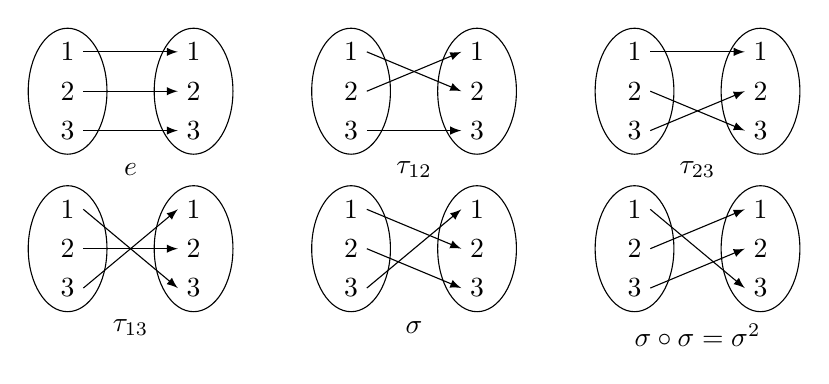
\begin{tikzpicture}
      \draw (0,0) ellipse (0.5cm and 0.8cm);
      \node at (0, 0.5) {1};
      \node at (0, 0) {2};
      \node at (0, -0.5) {3};
      \draw (1.6,0) ellipse (0.5cm and 0.8cm);
      \node at (1.6, 0.5) {1};
      \node at (1.6, 0) {2};
      \node at (1.6, -0.5) {3};

      \draw[-latex] (0.2, 0.5) -- (1.4, 0.5);
      \draw[-latex] (0.2, 0) -- (1.4, 0);
      \draw[-latex] (0.2, -0.5) -- (1.4, -0.5);

      \draw (3.6,0) ellipse (0.5cm and 0.8cm);
      \node at (3.6, 0.5) {1};
      \node at (3.6, 0) {2};
      \node at (3.6, -0.5) {3};
      \draw (5.2,0) ellipse (0.5cm and 0.8cm);
      \node at (5.2, 0.5) {1};
      \node at (5.2, 0) {2};
      \node at (5.2, -0.5) {3};

      \draw[-latex] (3.8, 0.5) -- (5, 0);
      \draw[-latex] (3.8, 0) -- (5, 0.5);
      \draw[-latex] (3.8, -0.5) -- (5, -0.5);

      \draw (7.2,0) ellipse (0.5cm and 0.8cm);
      \node at (7.2, 0.5) {1};
      \node at (7.2, 0) {2};
      \node at (7.2, -0.5) {3};
      \draw (8.8,0) ellipse (0.5cm and 0.8cm);
      \node at (8.8, 0.5) {1};
      \node at (8.8, 0) {2};
      \node at (8.8, -0.5) {3};

      \draw[-latex] (7.4, 0.5) -- (8.6, 0.5);
      \draw[-latex] (7.4, 0) -- (8.6, -0.5);
      \draw[-latex] (7.4, -0.5) -- (8.6, 0);

      \node at (0.8, -1) {$e$};
      \node at (4.4, -1) {$\tau_{12}$};
      \node at (8, -1) {$\tau_{23}$};

      \draw (0,-2) ellipse (0.5cm and 0.8cm);
      \node at (0, -1.5) {1};
      \node at (0, -2) {2};
      \node at (0, -2.5) {3};
      \draw (1.6,-2) ellipse (0.5cm and 0.8cm);
      \node at (1.6, -1.5) {1};
      \node at (1.6, -2) {2};
      \node at (1.6, -2.5) {3};

      \draw[-latex] (0.2, -1.5) -- (1.4, -2.5);
      \draw[-latex] (0.2, -2) -- (1.4, -2);
      \draw[-latex] (0.2, -2.5) -- (1.4, -1.5);

      \draw (3.6,-2) ellipse (0.5cm and 0.8cm);
      \node at (3.6, -1.5) {1};
      \node at (3.6, -2) {2};
      \node at (3.6, -2.5) {3};
      \draw (5.2,-2) ellipse (0.5cm and 0.8cm);
      \node at (5.2, -1.5) {1};
      \node at (5.2, -2) {2};
      \node at (5.2, -2.5) {3};

      \draw[-latex] (3.8, -1.5) -- (5, -2);
      \draw[-latex] (3.8, -2) -- (5, -2.5);
      \draw[-latex] (3.8, -2.5) -- (5, -1.5);

      \draw (7.2,-2) ellipse (0.5cm and 0.8cm);
      \node at (7.2, -1.5) {1};
      \node at (7.2, -2) {2};
      \node at (7.2, -2.5) {3};
      \draw (8.8,-2) ellipse (0.5cm and 0.8cm);
      \node at (8.8, -1.5) {1};
      \node at (8.8, -2) {2};
      \node at (8.8, -2.5) {3};

      \draw[-latex] (7.4, -1.5) -- (8.6, -2.5);
      \draw[-latex] (7.4, -2) -- (8.6, -1.5);
      \draw[-latex] (7.4, -2.5) -- (8.6, -2);

      \node at (0.8, -3) {$\tau_{13}$};
      \node at (4.4, -3) {$\sigma$};
      \node at (8, -3.1) {$\sigma \circ \sigma = \sigma^2$};
    \end{tikzpicture}
  \end{center}
  %kanske onöddigt att ha med detta nedan?
  Vi namnger dessa permutationer på liknande sätt som vi gjorde i förra avsnitt. Exempelvis så
  betyder $\tau_{13}$ att 1 mappas till 3 och vice versa medan allt annat mappas till sig självt.
  Lägg märke till att $\sigma^2 = \sigma \circ \sigma.$ Exponenten betyder alltså att man 
  \textbf{sammansätter} ett element $n$ gånger och \textbf{inte} multiplicerar, vilket 
  ibland kan vara vilseledande när symbolerna är heltal och $\circ$ defineras som addition.

  $Sym(M)$ är alla möjliga permutationer av $M$ och därför är 
  \[Sym(M) = S_3 = \{e, \tau_{12}, \tau_{23}, \tau_{13}, \sigma, \sigma^2\}.\]
  Även här kan man skapa en tabell likt Tabell 1 som gjordes i förra avsnittet. Vi hoppar 
  dock över detta. 

  Notera att $S_3$ inte är en abelsk grupp eftersom $\tau_{13} \circ \tau_{12} = \sigma$ medan
  $\tau_{12} \circ \tau_{13} = \sigma^2$ och att $|S_n|= n!$ 
  eftersom det första elementet kan mappas till 
  $n$ styckna element, det andra till $n-1$ element osv.
\end{exmp}
Vi kollar nu varför $S_n$ bildar en grupp.

% -----------------------------------
%-----------------VIKTIGT------------
% f
% https://www.math.kth.se/cirkel/2006/kompendium06.pdf
% LÄÄÄÄSSSSS
% -----------------------------------
%kanske gör en sats istället. Typ "sats 1.1: S_n är en grupp med operationen \circ. 
%Bevis \begin{enumerate} osv,...
\begin{enumerate}[I)]
  \item \textbf{Slutenhet.} Låt $P = f \circ g, \; f, g \in S_n$. 
  Enligt \hyperlink{kompbij}{sats 3.3.1} så är $P$ en permutation
  och eftersom $S_n$ innehåller alla möjliga permutationer så måste $P \in S_n$ och därför 
  uppfylls detta axiom. %du måste visa att f \circ g är en permutation, det vill säga en bijektion.
  %https://www.math.kth.se/cirkel/2006/kompendium06.pdf LÄS DENNA
  \item \textbf{Assosiativitet.} Detta axiom uppfylls enligt \hyperlink{ass}{sats 4.1.1}.
  \item \textbf{Enhetselementet.} Eftersom $S_n$ innehåller alla möjliga permutationer 
  så måste det finnas en permutation $e$ som mappar alla element till säg själva och 
  därför uppfylls detta axiom. 
  \item \textbf{Inverser.} Eftersom varje bijektion har en invers, 
  som enligt \hyperlink{invbij}{sats 3.3.2} också är en bijektion, så måste 
  $S_n$ innehålla dessa inverser och därför uppfylls detta axiom.
\end{enumerate}

\subsection{Cykliska grupper}
I detta del avsnitt kommer vi att kolla på cykliska grupper 
och diskutera vad addition av två heltal egentligen betyder, sätt från ett gruppteoretiskt 
perspektiv.

%skriv om definitionen.
%antigen ta bort <g> från definitionen eller ha med den och förklara.
%kommer <g> användes senare i texten? Om inte kan jag ta bort den. 
%ta bort exemplet om S_2 eller skriv om den. 

\subsubsection{Ändliga cykliska grupper}
%ändra kanske definitionen så att det bara finns symboler???
\begin{mydef}{Cykliska grupper}{}
  En \textit{cyklisk grupp} av ordning $n$, som betecknas $C_n$, är en grupp där varje element 
  kan uttryckas som $g^c$ för $g \in C_n$ och $c \in \mathbb{Z}.$ $g$ kallas för 
  \textit{grupp generatorn}. 
\end{mydef}
Det enklaste sättet att skapa och förstå cykliska grupper är att tänka på en klocka. 
För att konstruera till exempel $C_{12}$ så kan man lägga 12 symboler, till exempel 
$1, 2, \ldots, 12$, runt en cirkel. $C_{12}$ kommer då vara mägden av alla permutationer 
som "roterar" alla element. Figuren nedan visar en lämplig permutation som tillhör $C_{12}.$

\begin{center}
  \begin{tikzpicture}[line cap=rect,line width=1.5pt, scale = 0.8]
    \draw (0,0) circle [radius=2cm];
    \foreach \angle [count=\xi] in {60,30,...,-270}
    {
      \node[font=\large] at (\angle:1.60cm) {$\xi$};
      \node[scale = 2] at (\angle + 100:2.4cm) {
        $\mathbin{\rotatebox[origin=c]{\angle}{\vstretch{1.5}{\curvearrowright}}}$}; 
    }
  \end{tikzpicture}
\end{center}
1 blir alltså mappad till 2, 2 till 3 osv. Vi betecknar denna permutation med $\sigma$,
precis som förut. Vi kan även "rotera" alla element två gångder, $\sigma^2$,
och totalt elva gånger, $\sigma^{11}$. Vi kan uppenbarligen inte rotera överhuvudtaget 
och på så sätt få enhetselementet, $\sigma^0 = e.$
Notera att $\sigma^{12} = e$ och att allt repeteras efter tolv rotationer. 
Det finns alltså ingen anledning till att rotera mer än tolv gånger.

Vi skapar nu en mängd innehållande alla dessa permutationer, 
\linebreak
$C_{12} = \{e, \sigma, \sigma^2, \ldots, \sigma^{11}\}$. Varje element i $C_{12}$ kan
uttryckas som $\sigma^2$ för ett heltal $n$ och därför är denna grupp cyklisk med grupp generatorn $\sigma$.

Notera nu att 
%kanske ta bort detta nedan. jag använder mig av addition för att förklara vad det är...
%vilket inte är det bästa man kan göra. 
\[\sigma^n \circ \sigma^m = 
\underbrace{\sigma \circ \sigma \circ, \ldots, \circ \sigma}_{\text{$n + m$}} = \sigma^{n+m}.\]
$\sigma$ och $\circ$ är ju bara symboler som vi har hittat på och vi kan ändra dem när som helst. 
Varför inte beteckna $\sigma^n$ som $n$? $\sigma^2$ blir alltså 2 och $\sigma$ blir 1. 
Det finns inte heller något som stoppar oss från att kalla $\circ$ för addition och beteckna den 
med $+$ istället. Med dessa nya beteckningar så blir
%ändra kanske detta nedan. Det känns jätte självklart och jag kanske borde om formulera mig. 
$C_{12} = \{0, 1, 2, 3, \ldots, 11\}$ 
och vi ser att
% --------------------------------------------
%---------------VIKTIGT-----------------------
% --------------------------------------------
%rita kanske en cirkel som först utför \sigma^2 och sedan \simga^1 och visa visuellt 
%att 1 + 2 = 3. Men detta blir dock bara visuellt medan det jag har nu är mer generellt...
%Vad fan ska jag göra??????
\[\sigma^1 \circ \sigma^2 = \sigma^3 \iff 1 + 2 = 3\]
och att 
\[\sigma^{11} \circ \sigma^1 = e \iff 11 + 1 = 0.\]
Det som är så tjusigt med cykliska grupper är att moduloräkning trillar ut helt naturligt. 
Vi har, genom att ha konstruerat en cyklisk grupp av ordning tolv, 
sätt att modulo tolv egentligen är en konsekvens av 
att ha permuterat tolv element runt en cirkel. Notera att detta kan generaliseras till 
modulo $n$ genom att skapa en cyklisk grupp av ordning $n$, talet tolv var helt slumpmässigt.

Vi kollar nu varför alla cykliska grupper uppfyller gruppaxiomen. För detta så antar vi 
att gruppen $G$ är cyklisk med grupp generatorn $g$.
\begin{enumerate}[I)]
  \item \textbf{Slutenhet.} Eftersom $g$ är grupp generatorn så kan 
  $x, y \in G$ skrivas som $x = g^n, y = g^m$ för två heltal $n$ och $m$. 
  $g^n \circ g^m = g^{n + m}$ och eftersom 
  % g^n \circ g^m = g^c där c är kongruent med n + m modulo 12.
  $g$ är generatorn så måste $g^{n+m} \in G$. Notera att detta gäller även för $n+m > |G|$ eftersom 
  allt repeteras efter $g^{|G|}$ och därför uppfylls detta axiom.
  \item \textbf{Assosiativitet.} Detta axiom uppfylls enligt \hyperlink{ass}{sats 4.1.1}.
  \item \textbf{Enhetselementet.} Enhetselementet är permutationen som inte roterar något,
  $g^0.$
  \item \textbf{Inverser.} Inversen till $g^n$ för ett heltal $n$ är $g^{|G|-n}$ eftersom 
  $g^{n} \circ g^{|G|-n} = g^{|G|} = e$ och därför uppfylls detta axiom.
\end{enumerate}

\begin{exmp}
  Gruppen $S_2$ som med våra beteckningar defineras som $S_2 = \{e, \tau\}$ är 
  den cykliska gruppen $\mathbb{Z}_2$. Grupp generatorn är i detta fall 
  $\tau$ eftersom $\tau^2 = \tau \circ \tau = e$
  och genererar på så sätt hela gruppen.
\end{exmp}

%fundera och bevisa generellt på papper.
\begin{exmp}
  Mängden av de reella och komplexa lösningarna, som visas i figuren nedan,
  till ekvationen $z^5 = 1$ bildar en cyklisk grupp under operationen multiplikation.
  
  \begin{center}
    \begin{tikzpicture}
      \draw[-latex] (-2, 0) -- (2, 0) node[below] {$Re$};
      \draw[-latex] (0, -2) -- (0, 2) node[right] {$Im$};
      
      \draw[fill] (1, 0) circle [radius=1pt];
      \draw[fill] (0.309, 0.9510565) circle [radius=1pt];
      \draw[fill] (-0.809, 0.5877852) circle [radius=1pt];
      \draw[fill] (-0.809, -0.5877852) circle [radius=1pt];
      \draw[fill] (0.309, -0.9510) circle [radius=1pt];

      \draw[blue] (0.309, 0.9510565) -- (-0.809, 0.5877852);
      \draw[blue] (-0.809, 0.5877852) -- (-0.809, -0.5877852);
      \draw[blue] (-0.809, 0.5877852) -- (-0.809, -0.5877852);
      \draw[blue] (-0.809, -0.5877852) -- (0.309, -0.9510);
      \draw[blue] (1, 0) -- (0.309, 0.9510565);
      \draw[blue] (1, 0) -- (.309, -0.9510);
    \end{tikzpicture}
  \end{center}
  Mängden av lösningarna till $z^5 = 1$ är
  \[ L = \left\{ 
  1, \; 
  \pm \left( \cos \left( \frac{2 \pi}{5} \right) + i \sin \left( \frac{2 \pi}{5} \right) \right), \;
  \pm \left( \cos \left( \frac{4 \pi}{5} \right) + i \sin \left( \frac{4 \pi}{5} \right) \right)
  \right\} \]
  vilket enkelt kan visas genom att använda de Moivres formel. Vi ser att
  $z_2 = 
  \pm \left( \cos \left( \frac{2 \pi}{5} \right) + i \sin \left( \frac{2 \pi}{5} \right) \right)$
  genererar hela grupper eftersom $L = \{ z_2^0, z_2^1, z_2^2 \}$. $(L, \cdot)$ är cyklisk 
  %skriv om detta.
  och därmed också en grupp. Detta gäller för alla lösningar till ekvationen 
  på typen $z^n = 1$ under operationen multiplikation
  och en bra övning är att bevisa detta. 
\end{exmp}

\subsubsection{Oändliga cykliska grupper}
Skillnaden mellan ändliga cykliska grupper och oändliga cykliska grupper är 
hur många element som permuteras. 
När vi kollade på ändliga grupper så roterade vi ändligt många element. 
Med ändligt många element så finns det alltid ett sista element
som kan bli mappad till något, 
vilket gjorde att alla element slutligen roterar ett helt varv
efter repeterande permutatiner.
Tack vare detta så behöver man inte ha några direkta inverser som roterar elementen 
åt andra hållet. 

Vid fallet med oändliga cykliska grupper så finns det inget sista element. 
Tillföljd av detta så är det nödvändigt 
med direkta inverser som roterar åt motsatt håll för att alla gruppaxiom skall uppfyllas. 
På grund av detta faktum så blir det lite vilseledande om vi fortsätter rita cirklar. 
Vi ritar därför två tallinjer på varandra istället där den översta innehåller symbolerna 
som skall permuteras och där den
nedersta visar vart alla element mappas till 
efter en rotation.

\begin{center}
  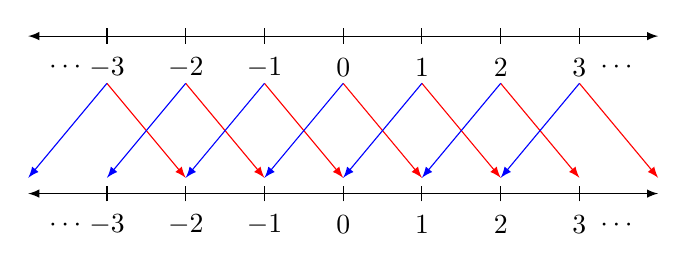
\begin{tikzpicture}
    \draw[latex-latex] (-4,0) -- (4,0);
    \foreach \x in  {-3,-2,...,3}
    {
      \draw (\x,0.1) -- (\x,-0.1);
      \node at (\x, -0.4) {$\x$};
      \draw[-latex, red] (\x, -0.6) -- (\x + 1, -1.8);
      \draw[-latex, blue] (\x, -0.6) -- (\x - 1, -1.8);
    }

    \draw[latex-latex] (-4,-2) -- (4,-2);
    \foreach \x in  {-3,-2,...,3}
    {
      \draw (\x,-2.1) -- (\x,-1.9);
      \node at (\x, -2.4) {$\x$};
    }

    \node at (-3.5, -0.4) {$\cdots$}; 
    \node at (3.5, -0.4) {$\cdots$}; 
    \node at (3.5, -2.4) {$\cdots$}; 
    \node at (-3.5, -2.4) {$\cdots$}; 
  \end{tikzpicture}
\end{center}
De röda pilarna i figuren ovan visar permutationen $\sigma$ och de blåa visar $\sigma^{-1}$.
Vi kan givetvis rotera flera gånger och, som tidigare nämnts, så är vi inte begränsade
till hur många gånger vi roterar. 
Den oändliga cykliska gruppen, som vi i denna text kommer att beteckna med $C$, är per definition 
\[C = \{ \sigma^n \; | \; n \in \mathbb{Z} \} = 
\{ \sigma, \sigma^{-1}, \sigma^2, \sigma^{-2}, \ldots \}.\]
Precis som förut så kan vi ändra våra beteckningar till något mer passande. 
Vad sägs om att beteckna $\sigma^n$ med $n$ och $\circ$ med $+$? 
Det är redan uppenbart från tidigare avsnitt att 
\[\sigma^5 \circ \sigma^3 = \sigma^8\]
och med våra nya beteckningar så kan följande ekvivalenta formulering ställas upp
\[5 + 3 = 8\]
vilket naturligtvist gäller inom den elementära algebran. 
Hela syftet som försöks framföras är att gruppteorin ger en alternativ synpunkt till vad 
tal egentligen är. Tal är i detta fall 
inte några tråkiga symboler och inte heller ett mått på hur många 
saker man har, utan istället permutationer. Addition, +, definerade vi som komposition, $\circ$,
och komposition som den resulterande permutationen efter att ha tillämpat två permutationer 
efter varandra. Men man kan ju definera $\circ$ precis som man önskar! 
Gruppen av heltal under operationen +, som alla använder dagligen, är alltså endast 
en infinitesimal skiva av det som finns att utforska inom gruppteorin. 

Notera dock att detta sätt att \textit{se} tal på är ifrån ett gruppteoretiskt perspektiv. 
Vi har egentligen inte definerat heltalen samt addition och om man vill ha formella och strikta definitioner så kan man läsa igenom \textit{Peanos axiom} som 
innehåller många axiom för de naturliga talen. 
Peanos axiom har varit väldigt viktig 
för forskning inom konsistens och fullständighet inom talteorin och kommer att betjäna 
de intresserade läsarna som söker efter mer rigorösa definitioner.

%ta kanske upp varför oändliga cykliska grupper uppfyller grupopaxiomen. Kanskde inte 
%nödvändigt tho. 

\subsection{Dihedrala grupper}

\subsection{Delgrupper}
\begin{mydef}{Delgrupper}{}
  En \textit{delgrupp} $H$ av gruppen $G$ är en delmängd av $G$ som också är en grupp och vi 
  skriver $H \le G$. Om $H \le G$ och $H \neq G$ så är $H$ en \textit{äkta delgrupp} av $G$
  och vi skriver $H < G$.
\end{mydef}
Lägg märkte till att varenda grupp $G$ har minst två delgrupper, den triviala delgruppen 
$\{e\} = S_1$ och $G$.
\begin{exmp}
  Den cykliska gruppen av ordning tre är en delgrupp av den symmetriska gruppen på tre element
  under operationen komposition $\circ$,
  $C_3 < S_3$. Detta eftersom $C_3 \subset S_3$ och $C_3$ bildar en grupp 
  under operationen $\circ$ enligt tidiare resultat.
  %"bildar en grupp enligt tidiare resultat" ändra detta till någon sats om jag ska ändra runt allt.
  %"enligt sats..."
\end{exmp}
\begin{exmp}
  $c \mathbb{Z} = \{cz \; | \; z \in \mathbb{Z}\} \le \mathbb{Z}$ (där $cz$ betyder 
  att vi multiplicerar $c$ med $z$) för ett heltal $c$ under operationen 
  addition. 
  Detta eftersom $c \mathbb{Z} \subseteq \mathbb{Z}$ och $c \mathbb{Z}$ bildar en 
  grupp under addition, vilket läsaren får lov att visa.
\end{exmp}
%nedan kan vara fristående appendix.
Det visar sig faktiskt att alla delgrupper till gruppen $(\mathbb{Z}, +)$ 
är på formen $c \mathbb{Z}$, vilket vi nu skall visa. 
\begin{mytheo}{}{}
  Alla delgrupper till gruppen $(\mathbb{Z}, +)$ 
  är på formen $c \mathbb{Z}, c \in \mathbb{Z}$.
\end{mytheo}
\begin{proof}
  Låt $H \le \mathbb{Z}$ under operationen addition. 
  Eftersom $H$ är en delgrupp till $\mathbb{Z}$ så gäller, per definition, att 
  $H \subseteq \mathbb{Z}$ och att $(H, +)$ bildar en grupp. 
  Eftersom $H$ är en delmängd av $\mathbb{Z}$ så finns det två olika fall för $H$.
  \begin{enumerate}[I)]
    \item $H$ kan vara den triviala delgruppen, det vill säga $H = \{0\}$. 
    \item $H$ är inte den triviala delgruppen.
  \end{enumerate}
  Om I) gäller så är $H = 0 \mathbb{Z}$ och alltså på formen $c \mathbb{Z}$ och beviset är 
  slutfört.
  
  Om II) gäller så måste $H$ innehålla både positiva och negativa heltal för att 
  gruppaxiomet "Inverser" skall uppfyllas. Detta medför att det måste finnas 
  ett minsta positiva heltal i $H$, vilket vi kan kalla för $b$.
  Vi visar nu att $H = b \mathbb{Z}$, 
  vilket är ekvivalent med att visa att $H \subseteq b \mathbb{Z}$
  och att $b \mathbb{Z} \subseteq H.$

  Vi visar först att $b \mathbb{Z} \subseteq H.$   
  Eftersom $H$ är en grupp och $b \in H$ så måste 
  även $nb \in H$ för ett naturligt tal $n$ enligt gruppaxiomet "Slutenhet". 
  Vidare har vi även att $-nb \in G$ enligt gruppaxiomet "Inverser".
  Eftersom 
  $b \mathbb{Z} = \{bz \; | \; z \in \mathbb{Z}\}$ så gäller $b \mathbb{Z} \subseteq H.$

  Det som återstår att visa är att $H \subseteq b \mathbb{Z}$. Vi antar motsatsen, 
  $H \not\subseteq b \mathbb{Z}$. Detta betyder att det existerar ett 
  $a \in H$ så att $a \notin b\mathbb{Z}.$ Eftersom $a \notin b\mathbb{Z}$ så 
  kan $a$ skrivas som $zb + r$ för $b > r > 0$, vilket betyder 
  att $r = a + (-zb)$. $a \in H$ och eftersom $-zb \in b \mathbb{Z}$ och $b \mathbb{Z} \subseteq H$ 
  så måste
  $-zb \in H$, vilket medför att $r \in H$ enligt gruppaxiomet "Sluthet". Villkoret $b > r > 0$ ger oss att $r$ är mindre än $b$, vilket är en motsägelse och därför 
  måste $H \subseteq b \mathbb{Z}$.
  
  Eftersom $H \subseteq b \mathbb{Z}$ samtidigt som $b \mathbb{Z} \subseteq H$ så måste 
  $b \mathbb{Z} = H$ och $H$ är alltså på den önskade formen.
\end{proof}



%skriv kanske inte något på dihedrala grupper, onödigt...

%------------------VIKTIGT---------------------------
%ändra "mappas" eller "map" och använd avbildning istället
\subsection{Grupp Homomorfism}
\begin{mydef}{Grupp Homomorfism}{}
  Låt $(G, \circ)$ och $(G', \cdot)$ vara grupper. 
  En \textit{grupp homomorfism} är en funktion $\varphi$ från $G$ till $G'$ som 
  uppfyller följande villkor
  \[\varphi (x \circ y) = \varphi (x) \cdot \varphi (y) \; \forall x, y \in G.\]
\end{mydef}

\begin{center}{}
    \begin{tabular}{c | c c c}
      $\circ$ &  & $y$ &\\
      \cline{1-4}
      &  &  & \\
      $x$ &  & $x \circ y$ & \\
      &  &  & \\
    \end{tabular} 
    \quad
    \begin{tikzpicture}
      % \node[font=\large] at (0.5, -0.2) {$\varphi : G \rightarrow G'$};
      \draw[-latex] (0, -1) -- (1.5, -1) node[font=\large] at (0.75, -0.7) {$\varphi$};
    \end{tikzpicture}
    \quad
    \begin{tabular}{c | c c c}
      $\cdot$ &  & $\varphi(y)$ &\\
      \cline{1-4}
      &  &  & \\
      $\varphi(x)$ &  & $\varphi(x) \cdot \varphi(y)$ & \\
      &  &  & \\
    \end{tabular} 
\end{center}
%kanske ändra definitionen eller ändra detta nedan. Jag måste föklara bättre.
Figuren ovan illusterar en homomorfism mellan två grupper som representeras av tabeller.
Homomorfism är alltså ett sätt att jämföra två gruppers algebraiska struktur. 

\hypertarget{exmp4.7}{}
\begin{exmp}
  Låt $G$ vara gruppen av de reella talen under addition och $G'$ vara gruppen av de reella 
  talen under multiplikation. $\varphi$ från $G$ till $G'$ som defineras 
  av $\varphi(x) = e^x$ är då en homomorfism eftersom
  \[\varphi(x + y) = e^{x+y} = e^x \cdot e^y = \varphi(x) \cdot \varphi(y).\]
\end{exmp}

\begin{mytheo}{}{}
  Låt $(G, \circ)$ och $(G', \cdot)$ vara grupper och 
  $\varphi: G \rightarrow G'$ en homomorfism. Då gäller 
  \begin{enumerate}[I)]
    \item $\varphi(e_G) = e_{G'}$ där $e_G$ är enhetselementet i $G$ och $e_{G'}$ är
    enhetselementet i $G'$.
    \item $(\varphi(x))^{-1} = \varphi(x^{-1}) \ \forall x \in G.$
  \end{enumerate}
\end{mytheo}
\begin{proof}
  I). Eftersom $\varphi$ är en homomorfism så gäller 
  \begin{align*}
    \varphi (e_G \circ y) &= \varphi (e_G) \cdot \varphi (y) \iff \\
    \varphi (y) &= \varphi (e_G) \cdot \varphi (y)
  \end{align*}
  för $y \in G.$ I högerledet komponerar vi $\varphi (e_G)$ med $\varphi (y)$ för att få tillbaka 
  $\varphi (y)$. $\varphi (e_G)$ agerar alltså som enhetselementet och därför måste 
  $\varphi (e_G) = e_{G'}.$

  II). Notera först att $(\varphi(x))^{-1}$ är inversen till $\varphi(x)$. 
  Eftersom $\varphi$ är en homomorfism så gäller
  \begin{align*}
    \varphi (x \circ x^{-1}) &= \varphi (x) \cdot \varphi (x^{-1}) \iff \\
    \varphi (e_G) &= \varphi (x) \cdot \varphi (x^{-1})
  \end{align*}
  och enligt I) får vi
  \[e_{G'} =\varphi (x) \cdot \varphi (x^{-1}).\]
  för $x \in G.$
  $\varphi (x^{-1})$ och $(\varphi(x))^{-1}$ är alltså båda inverser till $\varphi (x)$
  och eftersom det endast existerar en invers för varje element i en grupp så måste 
  $\varphi (x^{-1}) = (\varphi(x))^{-1}.$
\end{proof}

\begin{mydef}{Kärnan och bilden av en homomorfism}{}
  Låt $G$ och $G'$ vara grupper och $\varphi : G \rightarrow G'$ en homomorfism.
  \textit{Kärnan} av $\varphi$ betecknas $ker(\varphi)$
  och ges av 
  \[ker(\varphi) = \{g \in G \; | \; \varphi(g) = e_{G'}\}.\]
  \textit{Bilden} av $\varphi$ betecknas med $Im(\varphi)$ och ges av 
  \[Im(\varphi) = \{\varphi(g) \; | \; g \in G\}.\]
  På engelska kallas kärnar för \textit{kernel} och bilden för \textit{image}, varifrån 
  förkortningarna härstammar.
\end{mydef}
Kärnan av en homomorfism är alltså alla element i definitionsmängden som blir mappade 
till enhetselementet i målmångden och bilden av en homomorfism kan tänkas vara värdemängden. 
Figuren nedan visar vad alla dessa nya begrepp betyder visuellt.
\begin{center}
  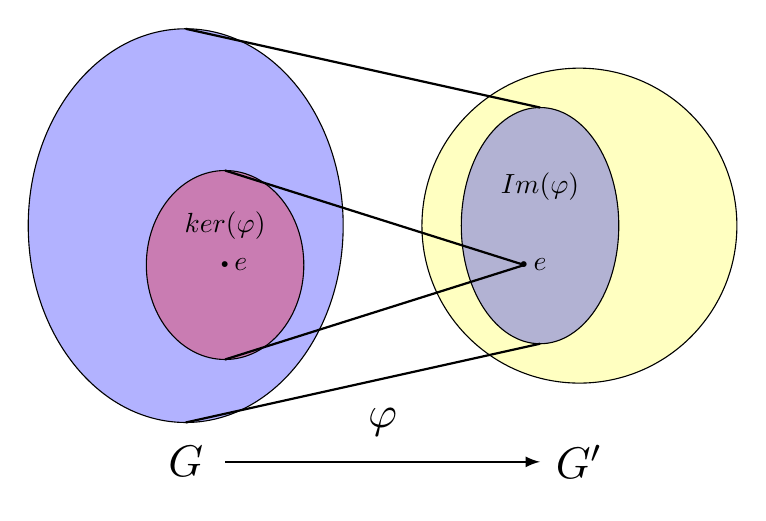
\begin{tikzpicture}
    \begin{scope} [fill opacity = .3]
      \draw[fill = blue] (-2.5,0) ellipse (2 and 2.5);
      \draw[fill = myblue] (2.5,0) circle (2);
      \draw[fill = blue] (2,0) ellipse (1 and 1.5) node[opacity=1] at (2, 0.5) {$Im(\varphi)$}
      node[opacity = 1] at (2, -0.5) {$e$} node[opacity = 1, scale=2] at (1.8, -0.5) {$.$};
      \draw[fill = red] (-2,-0.5) ellipse (1 and 1.2) node[opacity = 1, scale=2] at (-2, -0.5) {$.$}
      node[opacity = 1] at (-1.8, -0.5) {$e$} node[opacity = 1] at (-2, 0) {$ker(\varphi)$};
    \end{scope}

    \draw[thick] (-2.5, 2.5) -- (2, 1.5);
    \draw[thick] (-2.5, -2.5) -- (2, -1.5);

    \draw[thick] (-2, 0.7) -- (1.8, -0.5);
    \draw[thick] (-2, -1.7) -- (1.8, -0.5);
    % \draw[help lines](-5,5) grid (5,-6); 

    \node[scale = 1.6] at (-2.5, -3) {$G$};
    \node[scale = 1.6] at (2.5, -3) {$G'$};
    \draw[-latex, thick] (-2, -3) -- (2, -3) node[scale = 1.6] at (0, -2.5) {$\varphi$};
  \end{tikzpicture}
\end{center}

Det visar sig nämligen att för en homomorfism $\varphi : G \rightarrow G'$ så gäller
$Im(\varphi) \le G'$ och $ker(\varphi) \le G$. Eftersom det redan är uppenbart att
$Im(\varphi) \subseteq G'$
%kanske bevisa detta nedan ändå, eller??
och att $ker(\varphi) \subseteq G$ så behöver man alltså bara visa att kärnan och bilden bildar 
grupper. Detta utelämnas dock i denna text och läsaren får med glädje visa detta på egen hand.

Det som är viktigt med detta resultat är att vi kan tänka på alla injektiva homomorfier som
surjektiva också genom att begränsa målmängden till endast bilden. Säg till exempel att 
$\varphi : G \rightarrow G'$ är en injektiv homomorfism. För att göra $\varphi$ surjektiv och injektiv 
så kan man ändra målmängden till $Im(\varphi)$ så att $\varphi : G \rightarrow Im(\varphi)$.
Helt visuellt så betyder detta att vi tar bort det gula området 
(som innehåller alla element som inte är mappade till något i definitionsmängden) i figuren ovan.


%normala delgrupper här?? Kanske inte ens ha med dem.

\subsubsection{Grupp isomorfism}
\begin{mydef}{Isomorfism}{}
  En \textit{grupp isomorfism} är en grupp homomorfism som är bijektiv. 
  Om två grupper, $G$ och $G'$, är 
  isomorfa skriver vi $G \cong G'$.
\end{mydef}
Notera att varje isomorfism är en homomorfism men 
varje homomorfism behöver inte vara en isomorfism. 
Eftersom en isomorfism är en bijektion så är två gruppers algebraiska struktur identiska 
om de är isomorfa. Detta betyder att två isomorfa grupper endast skiljer sig åt symbol mässigt. 
Man kan alltså ändra sina symboler i den ena gruppen för att få den andra, vilket är den informella 
definitionen av isomorfism.


\begin{exmp}
Tidigare i texten har vi sätt att vi kan få gruppen av heltal under addition genom att 
ändra våra beteckningar i den oändliga cykliska gruppen. Detta betyder att 
den oändliga cykliska gruppen under komposition och heltalen under addition är isomorfa.
Mer formellt så är $C \cong \mathbb{Z}$ eftersom homomorfismem
$\varphi: C \rightarrow \mathbb{Z}$ 
som defineras av 
$\varphi (\sigma^n) = n$
är en bijektion.
\end{exmp}

\begin{exmp}
  I \hyperlink{exmp4.7}{exempel 4.7} hade vi den injektiva homomorfismem 
  \linebreak
  $\varphi : (\mathbb{R}, +) \rightarrow (\mathbb{R}, \cdot)$ som definerades av 
  $\varphi(x) = e^x.$ För att göra $\varphi$ bijektiv, och på så sätt göra den till en isomorfism, 
  så kan 
  vi ändra målmängden, $\mathbb{R}$, till bilden, $Im(\varphi)$. Eftersom $e^x, x \in \mathbb{R}$
  alltid är positiv så är $Im(\varphi)$ alla positiva reella tal, $\mathbb{R}^+.$
  Genom att begränsa målmängden till bilden så tar vi bort alla element som inte blir 
  mappade till något i definitionsmängden och därför är 
  $\varphi : (\mathbb{R}, +) \rightarrow (\mathbb{R}^+, \cdot)$ en isomorfism. 
\end{exmp}

\subsection{Cayleys sats}
Vi har redan sätt att vi kan konstruera en grupp busenkelt genom att använda permutationer
och majoriteten av alla grupper som har tagits upp har varit permutationsgrupper. Men 
\hyperlink{def4.1}{definitionen} nämner dock inget om permutationer och därför 
kan det kännas som vi endast har kollat på ett specialfall av grupper. Det är precis nu 
Cayles sats, som påstår att varje grupp kan tänkas som en permutationsgrupp, kommer till hands. 
Eftersom varje grupp kan tänkas som en permutationsgrupp så kan vi alltså endast kolla 
på permutationsgrupper utan att förlora generalitet.

För att bevisa denna viktiga sats så observerar vi följande.
\begin{enumerate}
  \item Alla delgrupper till $S_n$ är permutationsgrupper eftersom $S_n$ 
  innehåller alla möjliga permutationer på $n$ element.
  \item Att påstå att varje grupp kan "tänkas" som en permutationsgrupp är ekvivalent 
  med att påstå att varje grupp är isomorfisk med en permutationsgrupp.
\end{enumerate}
Med hjälp av 1 och 2 kan vi omformulera Cayles sats så att den blir lättare att bevisa. 
\begin{mytheo}{Cayleys sats}{}
  Varje grupp $G$ är isomorfisk med en delgrupp av $Sym(G)$.
\end{mytheo}
\begin{proof}
  Definera gruppen $(G, \cdot)$ och låt $\lambda_x: G \rightarrow G$ vara en funktion som 
  defineras av $\lambda_x (g) = x \cdot g$ för $x, g \in G$. 
  $\lambda_x$ är injektiv eftersom $\forall a, b \in G, \lambda_x(a) = \lambda_x (b) \implies
  x \cdot a = x \cdot b \implies x^{-1} \cdot x \cdot a = x^{-1} \cdot x \cdot b \implies a = b.$
  Dessutom är $\lambda_x$ surjektiv eftersom vi alltid kan hitta ett $b \in G$ så att 
  $a = \lambda_x(b)$ för alla $a \in G$, nämligen $b = x^{-1} \cdot a.$
  $\lambda_x$ är alltså en bijektion och eftersom $\lambda_x$ går från $G$ till $G$ så är 
  den, per definition, en permutation av $G$ och måste därför vara ett element i $Sym(G)$. 

  Definera mängden $H = \{\lambda_x \; |\; x \in G\; \}$ under operationen komposition, $\circ$.
  Härnäst visar vi att $H$ är en grupp.
  \begin{enumerate}[I)]
    \item \textbf{Slutenhet.} Låt $x, y, g \in G$, då gäller
    $(\lambda_x \circ \lambda_y)(g) = \lambda_x(\lambda_y(g)) = x \cdot y \cdot g = 
    \lambda_{x \cdot y}(g).$ Eftersom $G$ är en grupp så är $x \cdot y \in G$ vilket medför 
    att $\lambda_{x \cdot y} = \lambda_x \circ \lambda_y \in H$ och axiomet uppfylls.
    \item \textbf{Assosiativitet.} Detta axiom uppfylls enligt \hyperlink{ass}{sats 4.1.1}
    \item \textbf{Enhetselementet.} Enhetselementet är $\lambda_{e_G}$ där $e_G$ är 
    enhetselementet i $G$ och därför 
    uppfylls detta axiom. Detta eftersom $(\lambda_x \circ \lambda_{e_G})(g) = x \cdot e_G \cdot g
    = x \cdot g = \lambda_x (g)$ för $x, g \in G.$
    \item \textbf{Inverser.} Inversen till $\lambda_x$ är $\lambda_{x^{-1}}$ för $x \in G$
    och därför uppfylls detta axiom. 
    Detta eftersom, för $x, g \in G$, $(\lambda_x \circ \lambda_{x^{-1}})(g) = x \cdot x^{-1} \cdot g = 
    e_G \cdot g = \lambda_{e_G} (g)$ vilket är enhetselementet enligt III.
  \end{enumerate}
  Det är uppenbart att $H \subseteq Sym(G)$ och eftersom $H$ är en grupp så är $H$ en delgrupp 
  till $Sym(G)$. 

  Vi visar nu att $G \cong H$ för att slutföra beviset. Låt $\varphi: G \rightarrow H$ 
  vara en funktion definerad av $\varphi(x) = \lambda_x$. Notera att $\varphi$ direkt 
  blir surjektiv tillföljd av dess kontruktion och eftersom 
  $\forall x, y \in G, \varphi(x) = \varphi(y) \implies \lambda_x (g) = \lambda_y (g)
  \implies x \cdot g = y \cdot g \implies x = y$ för $g \in G$ så är även $\varphi$ injektiv. 
  Det som återstår att visa är att $\varphi$ är en homomorfism. För 
  $x, y \in G$ gäller $\varphi(x \cdot y) = \lambda_{x \cdot y}$. 
  Notera att $\lambda_{x \cdot y} (g) = x \cdot y \cdot g = (\lambda_x \circ \lambda_y)(g)$ 
  vilket betyder att $\varphi(x \cdot y) = \lambda_x \circ \lambda_y = \varphi(x) \circ \varphi(y)$
  och $\varphi$ är alltså en bijektiv homomorfism, det vill säga en isomorfism.
\end{proof}

\subsection{Sidoklasser och Lagranges sats}
%bevisa fermats lilla sats....
\begin{mydef}{}{Sidoklasser}
  Låt $(H, \circ)$ vara en delgrupp till $(G, \circ)$ och $a$ vara ett element i $G$. 
  Då är
  \[a \circ H = \{a \circ h \; | \; h \in H\}\]
  en \textit{vänstersidoklass} till $H$ med avseende på $a$ och 
  \[H \circ a = \{h \circ a \; | \; h \in H\}\]
  en \textit{högersidoklass} till $H$ med avseende på $a$. Ibland brukar $\circ$ utelämnas 
  och då skrivs $aH$ respektive $Ha$ istället.
\end{mydef}
\begin{exmp}
  Betrakta gruppen av heltal under addition och delgruppen $H = 3 \mathbb{Z}$ under addition. 
  Vänstersidoklassen till $H$ med avseende på 2 är då 
  $2 + 3 \mathbb{Z} = \{ 2+0, \;2+3, \;2+(-3), \;2+6, \;2+(-6), \ldots\}$.
  Eftersom $(\mathbb{Z}, +)$ är abelsk så gäller $2 + 3 \mathbb{Z} = 3 \mathbb{Z} + 2$. 
\end{exmp}

För att slippa kladdiga beräkningar kommer vi från och med nu utelämna opertationen och $ab$ kommer
skrivas istället för $a \circ b$.

\hypertarget{lemma4.1}{}
\begin{mylemma}{}{}
  Låt $G$ vara en grupp och $H$ en delgrupp till denna. Då gäller $hH = H = Hh$ samt 
  för $h \in H$.
\end{mylemma}
\begin{proof}
  Vi visar först att $hH = H$. 
  Ett godtyckligt element från $hH$ är på formen $hh'$ för $h' \in H$. Eftersom $H$ är 
  en delgrupp så måste $hh'$ vara ett element i $H$, vilket vilket visar att $hH \subseteq H$.

  Låt $g$ vara ett slumpmässigt element i $H$. $g = (hh^{-1})g$ och eftersom 
  $H$ är en delgrupp så gäller $g = (hh^{-1})g = h(h^{-1}g)$. Eftersom $h \in H$ så måste 
  $h^{-1} \in H$ och därför måste $g \in hH$, vilket visar att $H \subseteq hH$.

  Eftersom $H \subseteq hH$ och $hH \subseteq H$ så är $hH = H$. Argumentationen kan 
  replikeras för att visa $Hh = H$, vilket läsaren får gärna göra. 
\end{proof}

\hypertarget{lemma4.2}{}
\begin{mylemma}{}{}
  Låt $H < G$.
  Mängden av alla vänster (höger) sidoklasser av $H$ utgör en partition av $G$.
\end{mylemma}
\begin{proof}
  Vi visar först alla vänstersidoklasser av $H$ utgör en partition av $G$. 
  Eftersom alla element i $gH$ för $g \in G$ är på formen $gh$ för $h \in H$ så måste $gh \in G$
  och alltså gäller $gH \subseteq G$.

  Vi visar nu att två slumpmässiga vänstersidoklasser av $H$ är disjunkta.
  Låt
  $g, g' \in G, g \neq g'$ och anta att $gH$ och $g'H$ är olika. För att bevisa att 
  $gH \cap g'H = \emptyset$ så antar vi motsatsen, $gH \cap g'H \neq \emptyset$.
  Detta medför att det finns åtminstone ett element $x$ som finns i både $gH$ samt $g'H$ 
  och därför gäller
  \begin{align*}
    x &= gh, \; h \in H \\
    x &= g'h' \; h \in H.
  \end{align*}
  Detta medför att $gh = g'h' \iff g = (g'h')h^{-1} = g'(h'h^{-1})$ på grund av assosiativitet.
  $h'h^{-1}$ är ett element i $H$ vilket betyder att $g \in g'H$ och enligt 
  \hyperlink{lemma4.1}{lemma 4.8.1} så är $gH = g'H$, vilket är en motsägelse och därför 
  gäller $gH \cap g'H = \emptyset$.

  %ta kanske bort denna del. Onödigt. 
  Det är uppebart att $g \in gH$ för alla $g \in G$ och därför gäller 
  \[G = \bigcup \{gH \; |\; g \in G\}.\]
  Samma princip kan användas för att bevisa detta för mängden av alla
  \linebreak högersidoklasser.
\end{proof}

\hypertarget{lag}{}
\begin{mytheo}{Lagranges sats}{}
  Om $H$ är en delgrupp till en ändlig grupp $G$ så är ordningen av $H$ en delare till ordningen av 
  $G$, 
  $|G| = m |H|, \; m \in \mathbb{N}$.
\end{mytheo}
\begin{proof}
  Enligt \hyperlink{lemma4.2}{lemma 4.8.2} så bildar mängden av alla vänstersidoklasser
  till $H$ en 
  partition av $G$ och då gäller
  \[G = \bigcup \{gH \; |\; g \in G\} = g_1H \cup g_2H \cup \ldots \cup g_nH\]
  för $g_1, g_2, \ldots, g_n \in G.$
  Detta medför att 
  \[|G| = |g_1H| + |g_2H| + \ldots + |g_nH|\]
  och eftersom $|g_1H| = |H|$ så gäller 
  \[|G| = m |H|.\]
\end{proof}
\begin{mykol}{}{}
  En grupp med primtalsordning är en cyklisk grupp.
\end{mykol}
\begin{proof}
  Definera gruppen $(G, \circ)$ så att $|G| = p$ för något primtal $p$. Eftersom 
  $p > 1$ så finns det ett $g$ tillhörande $G$. Bilda den cykliska gruppen 
  $H = (\{g^z \; | \; z \in \mathbb{Z}\}, \circ)$. Eftersom $g \in G$ så $g^z \in G$ 
  för något heltal $z$ på grund av att $G$ är en grupp. $H$ är därför en delgrupp till $G$ och 
  ordningen av $H$ måste dela ordningen av $G$ enligt \hyperlink{lag}{Lagranges sats}.
  Ordningen av $H$ måste antigen vara 1 eller $p$, men eftersom $e, g \in H$ så måste 
  $|H| = p$. $|H| = |G|$ vilket betyder att $H = G$ och $G$ är således cyklisk.
\end{proof}

%ta kanske upp vad alla satser osv. är uppkallde efter. Kanske lite kul att veta detta också. 
\subsection{Gruppverkan och permutationsrepresentation}
Gruppverkan är en väldig viktig gren inom gruppteorin som också kommer att användas 
för att bevisa Banach-Tarski paradoxen. 
Tyvärr så kan denna del vara rätt så svårbegriplig och på grund av dess relevans 
kommer vi därför att gå igenom allt steg för steg för att verkligen gräva upp
de fundamentala ideerna bakom gruppverkan. 

%Skriv även att grupprepresentation ibland brukar användas för att definera 
%gruppverkan. 

%något inom stilen...
%Med hjälp av gruppverkan kan vi associera elementen i en grupp med permutationer,
%vilket också kan ses som gruppverkans syfte. 0

% I detta avsnitt kommer vi även kolla på varför det är relevant för en grupp homomorfism 
% att uppfylla ett specifikt villkor. 
%^kanske nämn detta i homomorfism delen istället. 
Tidiare har vi sätt att varje element i en grupp kan "tänkas" vara en permutation 
av en annan mängd. Men detta ger oss dock ingen nytta om vi inte har ett sätt 
att associera dessa element med permutationer på ett rimligt sätt.
Gruppverkan ger oss just denna associering mellan elementen och permutationer 
av en annan mängd, vilket också kan tänkas vara syftet med gruppverkan. 
Detta syfte framförs dock inte av definitionen och därför kan gruppverkan
tyckas vara svårbegriplig. 
När vi väl har förståt gruppverkan så kommer vi kunna ställa fram en ekvivalent formulering
till gruppverkan som är intuitivare och där syftet presenteras direkt i definitionen.

%Eftersom syftet inte framförs från definitionen kommer vi därför att spendera mycket 
%tid till att hitta syftet... eller något likande kanske. 

\begin{mydef}{Gruppverkan}{}
  En \textit{gruppverkan} av en grupp $G$ på en mängd $X$ är en funktion $f$ från den 
  kartesiska produkten av $G$ och $X$ till $X$, det vill säga $f: G \times X \rightarrow X$,
  som uppfyller följande axiom
  \begin{enumerate}[I)]
    \item $f(e_G, x) = x \; \forall x \in X$.
    \item $f(gh, x) = f(g, f(h,x)) \; \forall g, h \in G$ och $x \in X$.
  \end{enumerate}
  Funktionen $f(g, x)$ brukar skrivas som $g \cdot x$ och med denna notation 
  blir axiomen
  \begin{enumerate}[I)]
    \item $e_G \cdot x = x \; \forall x \in X$.
    \item $(gh) \cdot x = g \cdot (h \cdot x) \; \forall g, h \in G$ och $x \in X$.
  \end{enumerate}
\end{mydef}
Först och främst måste vi förstå vad en gruppverkan egentligen gör. 
Gruppverkan är en funktion som assocerar ett ordnat par $(g, x), \; g \in G, \; x \in X$
med ett element i mängden $X$. Helt intuitivt kan man tänka $f(g, x)$ eller 
$g \cdot x$ som en slags operation som sammansätter $g$ med $x$ för att få tillbaka ett 
element i $X$. Det är faktiskt precis så här man definerar en binär operation mer formellt. 

\begin{mydef}{Binär operation}{}
  En \textit{binär operation} på en mängd $X$ är en funktion $f: X \times X \rightarrow X$. 
\end{mydef}
En binär operation är alltså en funktion som mappar ett ordnat par med ett annat element 
i mängden. Om $f$ är den binära operationen addition så brukar vi dock inte skriva 
$f(1, 2) = 3$, utan vi har valt att skriva $1 + 2 = 3$ istället, vilket också 
är anledningen till varför man skriver $f(g, x)$ som $g \cdot x$ när man talar om gruppverkan. 

Notera att en binär operation sammansätter två element med varandra för att få tillbaka 
ett element i samma mängd och är därför sluten. Om $G$ är en grupp under en binär operation 
så uppfylls alltså gruppaxiomet Slutenhet direkt. På grund av detta så brukar 
axiomet Slutenhet helt utelämnas från definitionen. 
%skriv att om man nämner att gruppen är under en binär operation så behöver man inte 
%kolla på slutenhet. 

För att skapa en associering mellan elementen av en grupp $G$ och permutationer av 
en annan mängd $X$ så måste vi först skapa en funktion.
%just i steget nedan är precis det jag gör med permrep. Det är inte ett "intuitivare sätt"
%utan precis samma sak. 
Låt $f(g) = \sigma_g$ där 
$g \in G$ och där $\sigma_g$ är en permutation av mängden $X$. Följande sats visar 
att för $x \in X$ så är $\sigma_g(x) = g \cdot x$ en permutation av $X$. 

\hypertarget{sats4.9.1}{}
\begin{mytheo}{}{}
  $\sigma_g(x) = g \cdot x$ är en permutation av $X$.
\end{mytheo}
\begin{proof}
  Per definition så är $g \cdot x$ ett element av $X$ och därför går $\sigma_g$ från 
  $X$ till $X$. Eftersom en funktion som endast är injektiv eller surjektiv inte kan ha någon invers 
  så räcker det med att visa att $\sigma_{g^{-1}}$ är inversen till $\sigma_g$ 
  för att visa att $\sigma_g$ är en 
  bijektion. Nedan visar vi att $\sigma_{g^{-1}}(\sigma_g(x)) = x.$
  \[\sigma_{g^{-1}}(\sigma_g(x)) = \sigma_{g^{-1}}(g \cdot x) = g^{-1} \cdot (g \cdot x)\]
  och enligt axiomen får vi
  \[g^{-1} \cdot (g \cdot x) = (g^{-1}g) \cdot x = e_G \cdot x = x.\]
  På samma sätt kan man visa att $\sigma_g(\sigma_{g^{-1}}(x)) = x.$
  \[\sigma_g(\sigma_{g^{-1}}(x)) = g \cdot (g^{-1} \cdot x) = (g g^{-1}) \cdot x = x.\]
\end{proof}
Vi kan börja se varför axiomen inom gruppverkan är så viktiga. Utan dem skulle vi inte 
kunna associera element med permutationer och hela syftet med gruppverkan skulle försvinna. 

För att ta detta ett steg vidare kan vi nu skapa permutations gruppen 
$G' = \{\sigma_g \; | \; g \in G\}$ under komposition $\circ$ som kommer att agera som 
en "permutations variant" av $G$. Vi behöver naturligtvist också visa att $G'$ är en grupp
och detta görs nedan. 
\begin{enumerate}[I)]
  \item \textbf{Slutenhet.} För $g, h \in G$ och $x \in X$ gäller 
  $(\sigma_g \circ \sigma_h) (x) = \sigma_g(\sigma_h(x)) = \sigma_g(h \cdot x)$. Eftersom 
  $h \cdot x \in X$ så är $\sigma_g(h \cdot x) \in G'$ och axiomet uppfylls.
  \item \textbf{Assosiativitet.} Detta axiom uppfylls enligt \hyperlink{ass}{sats 4.1.1}
  \item \textbf{Enhetselementet.} Enhetselementet är $\sigma_{e_G}$ eftersom för 
  $g \in G$ och $x \in X$ så gäller $(\sigma_{e_G} \circ \sigma_g) (x) = 
  e_G \cdot (g \cdot x) = \sigma_g(x)$ och axiomet uppfylls. 
  \item \textbf{Inverser.} Om $g \in G$ så finns även $g^{-1}$ i $G$ och därför finns 
  $\sigma_{g^{-1}}$ i $G'$. Beviset av \hyperlink{sats4.9.1}{sats 4.9.1} visar 
  att inversen till $\sigma_g$ är $\sigma_{g^{-1}}$ och axiomet uppfylls. 
\end{enumerate}
Men för att $G'$ verkligen ska motsvara $G$ så måste deras "operationer överensstämma", det 
vill säga $\sigma_{gh} = \sigma_g \circ \sigma_h$ för $g, h \in G$.
Figuren nedan visar vad detta betyder visuellt.

\begin{center}{}
  \begin{tabular}{c | c c c}
     &  & $h$ &\\
    \cline{1-4}
    &  &  & \\
    $g$ &  & $gh$ & \\
    &  &  & \\
  \end{tabular} 
  \quad
  \begin{tikzpicture}
    % \node[font=\large] at (0.5, -0.2) {$\varphi : G \rightarrow G'$};
    \draw[-latex] (0, -1) -- (1.5, -1) node at (0.75, -0.7) {$f$} node at (-0.3, -1) {$G$}
    node at (1.8, -1) {$G'$};
  \end{tikzpicture}
  \quad
  \begin{tabular}{c | c c c}
    $\circ$ &  & $\sigma_h$ &\\
    \cline{1-4}
    &  &  & \\
    $\sigma_g$ &  & $\sigma_g \circ \sigma_h$ & \\
    &  &  & \\
  \end{tabular} 
\end{center}
Om $\sigma_{gh} \neq \sigma_g \circ \sigma_h$ så skulle det vara svårt att jämföra elementen i 
$G$ med $G'$ och eftersom vi strävar efter en koppling mellan dessa grupper så
är detta förhållande nödvändig. Satsen nedan bevisar detta. 

\hypertarget{sats.4.9.2}{}
\begin{mytheo}{}{}
  $\sigma_{gh} = \sigma_g \circ \sigma_h$.
\end{mytheo}
\begin{proof}
  Vi kollar på högerledet och jobbar oss fram till vänsterledet.
  \[H.L = (\sigma_g \circ \sigma_h)(x) = g \cdot (h \cdot x) = (gh) \cdot x = \sigma_{gh}(x) = V.L\]
  Notera användingen av axiom II.
\end{proof}

Sammanfattningsvis har vi skapat en grupp $G$ och med hjälp av gruppverkan 
skapat en "permutations variant" av denna grupp som vi kallad för $G'$. Med hjälp av 
detta kan vi gå fram och tillbaka mellan grupperna och välja om vi vill jobba 
med permutationer eller "vanliga element". För att göra saker och ting lite mer tydligare 
så kan vi tänka på $G$ som gruppen av heltal under addition. Vi har tidigare sätt 
att denna grupp är isomorfisk med den oändliga cykliska gruppen, som alltså är en 
permutationsgrupp. En lämplig "permutations variant" av gruppen av heltal under addition 
är därför den oändliga cykliska gruppen. 

För att ställa fram en ekvivalent formulering till gruppverkan med samma syfte 
så kan vi direkt skapa funktionen
$\varphi: G \rightarrow Sym(X)$
som defineras av $\varphi(g) = \sigma_g$.
I detta fall blir $G'$, som är "permutations varianten" av $G$, $Im(\varphi) = 
\{\sigma_g \; | \; g \in G\}$. Men, precis som vid \hyperlink{sats.4.9.2}{sats 4.9.2}, så 
vill vi skapa en koppling mellan $G$ och $G'$ och därför måste 
\[\sigma_{gh} = \sigma_g \circ \sigma_h\]
och per definition av $\varphi$ är detta ekvivalent med 
\[\varphi(gh) = \varphi(g) \circ \varphi(h).\]
Detta är nämligen villkoret som 
en funktion måste uppfylla för att den ska anses vara en homomorfism. Detta betyder att 
$\varphi$ måste vara en homomorfism. Det vi har gjort nu heter 
permutationsrepresentation och defineras nedan.

\begin{mydef}{Permutationsrepresentation}{}
  En \textit{permutationsrepresentation} av en grupp $G$ på en mängd $X$ 
  är en homomorfism från $G$ till den symmetriska gruppen av $X$:
  \[\varphi: G \rightarrow Sym(X).\]
\end{mydef}

Permutationsrepresentationer och gruppverkan är alltså starkt kopplade med varandra 
eftersom de delar samma syfte. Notera att vi gick från gruppverkan till grupprepresentation
och att vi kan gå baklänges och skapa en gruppverkan från en grupprepresentation. 
Vi kan alltså skapa den ena från den ena, vilket betyder att de två är ekvivalenta med varandra
och ibland brukar även visa texter definera gruppverkan precis så som vi definerade 
grupprepresentation.

Om vi minns tillbaka till Cayles sats, som påstår att varje grupp är isomorfisk med en delgrupp
av $Sym(G)$, så inser vi att det finns ett till sätt att bevisa den med hjälp av 
gruppverkan och permutationsrepresentationer. Eftersom de två är ekvivalenta så kan vi 
först visa att $G$ verkar på sig själv enligt $g \cdot g' = g \circ g'$ 
som då kommer skapa en homomorfism
$\varphi: G \rightarrow Sym(G)$ som defineras av $\varphi(g) = \sigma_g$
där $\sigma_g(g') = g \cdot g' = g \circ g'$. Sedan återstår det 
bara att visa att $\varphi$ är en injektion eftersom $G$ blir då isomorfisk med $Im(\varphi)$, 
som är en delgrupp av $Sym(G)$. Alla steg till beviset är upplagda för läsaren som nu 
borde kunna bevisa och förstå detta på egen hand. 
%kanske strunta i stegen. Blir kanske bättre om läsaren får klura ut detta på egen hand. 

%skriv om faithful groups. 
%skriv att cayles sats kan bevisas genom gruppverkan. 
%exempel: C_4 verkar på Z_4 genom sigma^n \cdot x = n + m.

% Vi har sätt att det oftast blir lättare att tänka på grupper som permutationsgrupper, 
% men just i detta fall blir det bäst om vi tänker på gruppen $G$ som en "vanlig" 
% grupp utan permutationer (som t.ex. gruppen av heltal under addition). 


%ändra massor av skit här. 
% ------------------------------
%---------------VIKTIGT---------------
%Gruppverkan hjälper oss att skapa ett sätt att associera element med permutationer. 
%Detta är dock kanske inte HELA syftet med gruppverkan utan kan ses som ett hjälpmedel. 
%Permutations representationer (det vill säga min andra definition) är ett då ett annat sätt 
%att göra precis det som gruppverkan gör. De två är alltså kopplade med varandra: 
%Om jag har den ena kan jag få den andra och vice versa. Gruppverkan och Perm.rep. 
%är alltså två olika saker som hjälper oss att skapa något som är användbart. 
% ------------------------------
\begin{exmp}
  Betrakta gruppen $Sym(M)$ under komposition $\circ$ där 
  $M = \{1, 2, 3\}$. $Sym(M)$ verkar då på mängden $M$
  genom funktionen $g \cdot x = g(x)$, eller om man så vill $f(g, x) = g(x)$, 
  där $g \in G$ och $x \in M$. Detta eftersom båda axiomen uppfylls:
  \begin{enumerate}[I)]
    \item $e_G \cdot x = e_G(x) = x$ för alla $x \in M$.
    \item $(g \circ h) \cdot x = g(h(x)) = g \cdot h(x) = g \cdot (h \cdot x).$
  \end{enumerate}
  Sätt ifrån ett permutationsrepresentations perspektiv så är 
  $\varphi: Sym(M) \rightarrow Sym(M)$ definerad av $\varphi(g) = g, \; g \in Sym(G)$
  en homomorfism och därför måste $Sym(M)$ verka på $M$.
\end{exmp}

%ta bort denna. C verkar på Z genom sigma(z) = sigma cdot z, precis som i förra exemplet. 
\begin{exmp}
  Den oändliga cykliska gruppen $C$ under komposition $\circ$ verkar på alla heltal $\mathbb{Z}$
  genom funktionen $\sigma^n \cdot m = n + m$ för $n, m \in \mathbb{Z}$.
  Detta eftersom båda axiomen uppfylls:
  \begin{enumerate}
    \item $\sigma^0 \cdot m = 0 + m = m$.
    \item $(\sigma^n \circ \sigma^z) \cdot m = \sigma^{n + z} \cdot m = (n + z) + m = 
    \sigma^n \cdot (\sigma^z \cdot m)$.
  \end{enumerate}
  Sätt ifrån ett permutationsrepresentations perspektiv så är 
  $\varphi: C \rightarrow Sym(\mathbb{Z})$ definerad av $\varphi(\sigma^n) = \sigma^n, \; 
  n \in \mathbb{Z}$ en homomorfism och därför måste $C$ verka på $\mathbb{Z}$.
\end{exmp}

%tänk ut hur man tänka detta helt intuitivt och kolla varför just dessa axiomer används. 
%Koppla sedan allt till andra definitionen och säg att den är "bättre" att använda.

\subsubsection{Banor}
Med den förståelsen vi nu har om gruppverkan så kan vi ägna vår tid åt banor
\begin{mydef}{Banor}{}
  Om $G$ verkar på mängden $X$ och $x \in X$ är \textit{banan} för $x$ mängden 
  \[\orbit_x = \{g \cdot x \; | \; g \in G\}.\]
\end{mydef}
Tidigare har vi definerat funktionen $\sigma_g(x) = g \cdot x$ och även bevisat i 
\hyperlink{sats4.9.1}{sats 4.9.1} att 
denna är en permutation av $X$. Med denna definition kan vi uttrycka banan för $x$ som 
$\orbit_x = \{\sigma_g(x) \; | \; g \in G\}$ och 
således är ett elements bana mängden av alla möjliga destinationer under alla permutationer 
$\sigma_g$.

\begin{exmp}
  Om $M = \{1, 2, 3\}$ så verkar $Sym(M)$ under komposition $\circ$ på $M$ 
  genom funktionen $g \cdot x = g(x), \; g \in Sym(M), x \in M$ enligt tidigare resultat. Banan för 
  1 är då $\orbit_1 = \{g \cdot x \; | \; g \in Sym(M)\} = \{g(x) \; | \; g \in Sym(M)\}
  = \{1, 2, 3\}$ eftersom $Sym(M)$ innehåller alla möjliga permutationer på $M$.
  Detta betyder även att $\orbit_1 = \orbit_2 = \orbit_3$. För en visualisering så
  kan man kolla på figurerna i \hyperlink{exempel4.2}{exempel 4.2}.
\end{exmp}

\begin{exmp}
  Gruppen $G = \{e, \tau_{12}, \tau_{13}\}$ under komposition $\circ$ verkar på 
  mängden $M = \{1, 2, 3\}$ genom funktionen $g \cdot x = g(x), \; g \in G, x \in M$. 
  Banan för 2 är då $\orbit_2 = \{1, 2\}$ och banan för 1 är $\orbit_2 = \{1, 2, 3\}$.
\end{exmp}

\begin{mytheo}{}{}
  Låt $G$ vara en grupp som verkar på mängden $X$. Mängden av alla banor av $x \in X$
  utgör då en partition av $X$. 
\end{mytheo}
\begin{proof}
  $\orbit_x$ är en delmängd till $X$ eftersom $g \cdot x \in X$ för $g \in G$ och $x \in X$.
  Vi visar nu att mängden $\{\orbit_x \; | \; x \in X\}$ är parvis disjunkt. 
  Anta att $\orbit_x$
  och $\orbit_{x'}$ för $x' \in X$ inte är disjunkta. Då måste det finnas 
  ett element $y$ som finns i både $\orbit_x$ och $\orbit_{x'}$ och då gäller 
  \begin{align*}
    y &= g \cdot x \\
    y &= g' \cdot x'.
  \end{align*}
  för $g' \in G.$ Detta ger att 
  \begin{align*}
    g \cdot x &= g' \cdot x' \iff \\
    g^{-1} \cdot (g \cdot x) &= g^{-1} \cdot (g' \cdot x')
  \end{align*}
  och enligt axiomen får vi 
  \begin{align*}
    g^{-1} \cdot (g \cdot x) &= g^{-1} \cdot (g' \cdot x') \iff \\
    (g^{-1} g) \cdot x &= (g^{-1} g') \cdot x' \iff \\
    x &= (g^{-1} g') \cdot x'.
  \end{align*} 
  På samma sätt kan man visa att $x' = (g'^{-1}g) \cdot x$ genom att 
  "multiplicera" med $g'^{-1}$ på båda sidorna om $g \cdot x = g' \cdot x'$. 
  Eftersom $g^{-1} g'$ och $g'^{-1}g$ är båda element i $G$ så är 
  $x \in \orbit_{x'}$ samt $x' \in \orbit_x$ och därför är även $g \cdot x \in \orbit_{x'}$
  och $g \cdot x' \in \orbit_{x}$. Detta betyder att $\orbit_x \subseteq \orbit_{x'}$ och att 
  $\orbit_{x'} \subseteq \orbit_x$ vilket medför att $\orbit_x = \orbit_{x'}$.
  Eftersom två banor antigen är disjunkta eller identiska så gäller 
  \[\bigcap \{\orbit_x \; | \; x \in X\} = \emptyset.\]
\end{proof}

\section{Oändligheten}

\begin{center}
  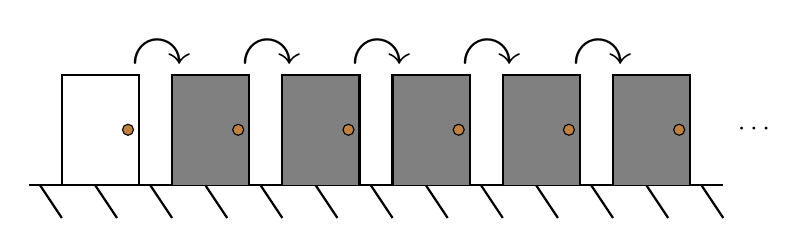
\begin{tikzpicture}[scale=1.4]
    % \draw (0,0,0) --  (2,0,0)  node[pos=1.05]{$x$};
    % \draw (0,0,0) -- (0,3,0) node[pos=1.05]{$y$};
    % \draw (0,0,0) -- (0,0,2) node[pos=1.1]{$z$};

    % \draw[thick] (-1.5, 0, -0.8) -- (0, 0, 0) -- (0, 2, 0) -- (-1.5, 2, -0.8) -- (-1.5, 0, -0.8);
    % \draw[thick] (0, 0, 0) -- (5, 0, -1.7);
    % \draw[thick] (5, 2, -1.7) -- (0, 2, 0);
    % \draw[thick] (3.5, 2, -2.5) -- (-1.5, 2, -0.8);
    % \node[font=\Large] at (5.5, 1, -2) {$\mathbin{\rotatebox[origin=c]{7}{$\cdots$}}$};

    \draw[thick] (-0.3, 0) -- (6, 0);
    \foreach \x in  {0, 0.5,...,6}{
      \draw[thick] (\x-0.2, 0) -- (\x, -0.3);
    }
    \node[] at (6.3, 0.5) {$\cdots$};

    \foreach \d in  {1,2,...,5}{
      \draw[thick, fill=gray] (\d, 0) -- (\d, 1) -- (\d + 0.7, 1) -- (\d + 0.7, 0);
      \draw[fill=brown] (\d + 0.6, 0.5) circle (0.05);
      \node[font=\Large, xscale=1.5, yscale=1.4] at (\d-0.1, 1.2) {$\curvearrowright$};
    }

    \draw[thick] (0, 0) -- (0, 1) -- (0.7, 1) -- (0.7, 0);
    \draw[fill=brown] (0.6, 0.5) circle (0.05);
  \end{tikzpicture}
\end{center}

\begin{mydef}{}{}
  In any right triangle, the area of the square whose 
  side is the hypotenuse is equal to the sum of the areas of
  the squares whose sides are the two legs.    
\end{mydef}

\begin{tcolorbox}[enhanced,center upper,size=fbox,drop shadow southeast,sharp corners, 
  colframe=black, colback=gray!30!white]
\begin{definition}
  In any right triangle, the area of the square whose 
  side is the hypotenuse is equal to the sum of the areas of
   the squares whose sides are the two legs.
\end{definition}
\end{tcolorbox}

\section{Banach-Tarski paradoxen}

\subsection{Urvalsaxiomet}
\subsection{Frigrupp med en generator}
\subsection{Frigrupp i \texorpdfstring{$SO_3$}{}}
\subsection{Banach-Tarski paradoxen i högre dimensioner}

\section{Diskussion}
\section{Slutsats}
\end{document}

%------------------VIKTIGT------------------
%FRÅGESTÄLLNING:::::: Kan en sfär i n dimensioner duplikeras?
%kan man på så sätt skapa en boll i en dimension större än den man började med??
%(t.ex. från 3d till 4d). Vad är det som orakar denna paradox? (denna fråga är dock trivial).
%kan detta hända i den riktiga världen?
%finns det ett enklare sätt att förstå detta utan att använda matte?
%https://en.wikipedia.org/wiki/N-sphere
https://en.wikipedia.org/wiki/Banach%E2%80%93Tarski_paradox#Obtaining_infinitely_many_balls_from_one'

%skriv även lite snabbt varför det inte går att duplikera en cirkel. 
% It leads to Bustany's Rule of Infinity: Infinity and Intuition do not mix.

%jag måste bevisa att skärningen mellan en platta, w=c, och en sfär i fyra dimensioner
%är en sfär i tre dimensioner. Sedan kan jag samla alla dessa 3d sfärar och dublicera dessa 
%och sammansätta dem till en ny 4d sfär. 

%kan jag skapa en 4d sfär från en 3d? Eftersom en 4d består av oändligt många 3d sfärar 
%(visa detta eller utgå bara från att skärningen mellan 4d och en platta blir 3d och bör 
%därför bestå av 3d) så kan jag bara dublicera oändligt många 3d sfärar och sedan sammansätta 
%dessa till en 4d. 

%Något annat coolt man kan skriva om??
%------------------VIKTIGT------------------